\documentclass[a4paper,12pt]{article}
\thispagestyle{empty}
\usepackage{graphicx}
\usepackage{geometry}
\geometry{a4paper,total={180mm,250mm},left=15mm,top=30mm}
\usepackage{fancyhdr}
\usepackage{adjustbox}
\usepackage{pdfpages}
\renewcommand{\thefigure}{\arabic{section}.\arabic{subsection}.\arabic{figure}}




\begin{document}
\begin{center}
\Large\textbf{\scshape A}\\
\Large\textbf{\scshape PROJECT REPORT}\\
\Large\textbf{\scshape ON}\\[1.5cm]
\vspace{0.1in}
\LARGE\textbf{“DESIGN OF SELF CHARGING ELECTRIC VEHICLE USING SOLAR AND WIND POWER"}\\[1.5cm]
\large\textbf{SUBMITTED BY}\\[0.5cm] 
HRUGVED MANBHEKAR \hspace{6.25cm} B150133832\\[0.15cm]
SHREYASH MODAK \hspace{7.5cm} B150133834\\[0.15cm]
SAURAV TAYADE \hspace{8cm} B150133856\\[1cm]
Under the guidance of\\[0.16cm]
\Large\textbf{Prof. R.R.KHINDE}\\[0.5cm]

\includegraphics[scale=0.5]{logo.jpg}\\
\Large\textbf{\scshape DEPARTMENT OF ELECTRONICS \& TELECOMMUNICATION ENGINEERING,}\\[0.75cm]
\Large\scshape\textbf{\scshape KARMAVEER KAKASAHEB WAGH INSTITUTE OF ENGINEERING EDUCATION AND RESEARCH, NASHIK.}\\[0.75cm]
\Large\textbf{\scshape SAVITRIBAI PHULE PUNE UNIVERSITY}\\[0.75cm]
\Large\textbf{\scshape 2021-2022}\\
\end{center}

%%%%%%%%%%%%%%%%%%%%%%%Dissertation Approval Sheet%%%%%%%%%%%%%%%%%%%%%%%%%%%%%
\newpage
\thispagestyle{empty}
\begin{center}
\Large\textbf{Dissertation Approval Sheet}\\[1cm]
\end{center}
\large This is to certify that the project work titled \textbf{“DESIGN OF SELF CHARGING ELECTRIC VEHICLE USING SOLAR AND WIND POWER”}, has been submitted in partial fulfillment of the Bachelor’s degree in Electronics Engineering during the academic year of 2021-2022 by following students:\\[2cm]
\begin{itemize}
\item HRUGVED MANBHEKAR {B150133832}\\
\item SHREYASH MODAK {B150133834}\\
\item SAURAV TAYADE {B150133856}\\[2cm]
\end{itemize}
\large This project confirms to the standards laid down by the Savirtibai Phule Pune University and has been completed in satisfactory manner as a partial fulfillment for the Bachelor’s degree in Electronics Engineering.\\[2in]
\begin{tabular}{c c c}
\textbf{External Examiner} & \hspace{0.15cm} \textbf{Internal Guide} & \hspace{0.15cm} \textbf{Head of Department}\\

               & \hspace{0.9cm}(Prof. R.R.Khinde)  & \hspace{1cm}(Prof. Dr.D.M.Chandwadkar)\\
\end{tabular}\\

%%%%%%%%%%%%%%%%%%%%%%%%%%%%ABSTRACT%%%%%%%%%%%%%%%%%%%%%%%%%%%%%%%

\newpage
\begin{center}
\textbf{\LARGE\scshape\underline{ABSTRACT}}\\[2cm]
\addcontentsline{toc}{section}{\numberline{}{ABSTRACT}}
\end{center}
\large To shift from Conventional Vehicles to Electric Vehicle, more charging time
is very important factor. So, recharging Electric Vehicle while driving
increases its efficiency. Nowadays, Solar and Wind Energy are wasted in
Electric Vehicle while driving. Thus, using this energy to recharge the
battery is one of the good solution for it. For this we are going to use Solar
panel, Wind turbines, BLDC motors, Recharge-able batteries,
Arduino/Microcontroller, Inverter, Rectifier, over charging avoiding circuits,
wheels, vehicle’s structure. The working, While the Electric Vehicle starts
moving with power motor placed at the rear part, the generator motor
generates the power with the moving wheels. At the same time wind mills
and solar panel generates the power to boost recharging. When the battery is
completely charged the power from other generators is cut using
Microcontroller programming. This Technology can also be applied to 3
wheelers and 4 wheelers, commercial vehicle and also in trains. The moto of
this project is to make Electric Vehicle self-sufficient in charging it, using
Wind and Solar Power.
%%%%%%%%%%%%%%%%%%%%ACKNOWLEDGEMENT%%%%%%%%%%%%%%%%%%%%%%%%%%%%%

\newpage
\begin{center}
\textbf{\LARGE\scshape\underline{ACKNOWLEDGEMENT}}\\[2cm]
\addcontentsline{toc}{section}{\numberline{}{ACKNOWLEDGEMENT}}
\end{center}
\large We would like to express our deep gratitude to \textbf{Prof. R.R.KHINDE} Sir  for his  patient guidance, enthusiastic involvement  and useful critiques of this project work. Our grateful thanks extends  to him for his advice and assistance in keeping our progress on schedule right from project synopsis to project report. We're very much thankful to him for encouraging us to acquire knowledge of \LaTeX \ system, which is a document preparation system for high-quality typesetting.\\

\large We would also like to extend our thanks to the technicians of the laboratory of the E\&TC department for their help in offering us the resources in running the program.\\

\vspace{4cm}
\begin{flushright}
1. Hrugved Manbhekar\\[1in]
2. Shreyash Modak\\[1in]
3. Saurav Tayade\\


\end{flushright}

%%%%%%%%%%%%%%%%%%%%%%%%TOC%%%%%%%%%%%%%%%%%%%%%%%%%%%%%%%%%%%%%
\newpage
\tableofcontents
\addcontentsline{toc}{section}{\numberline{}{Table of Contents}}
\newpage
\listoffigures
\addcontentsline{toc}{section}{\numberline{}{List of Figures}}



%%%%%%%%%%%%%%%%%%%%%%%%%%%%%%%%%%%%%%%%%%%%%%%%%%%%%%%%%%%%%%%

\newpage

\pagenumbering{arabic}
\pagestyle{fancy}
\fancyhf{}
\fancyhead[R]{“DESIGN OF SELF CHARGING ELECTRIC VEHICLE USING SOLAR AND WIND POWER"}
\fancyfoot[L]{Department of E\&TC}
\fancyfoot[R]{\thepage}
\renewcommand{\footrulewidth}{1pt}


%%%%%%%%%%%%%%%%%%%%%%%%%%%%%%%%%%%%%%%%%%%%%%%%%%%%%%%%%%%%%%%
\newpage
\thispagestyle{empty}
\vspace*{0.25\textheight}
\begin{center}
\begin{center}
{\bfseries\LARGE <------------------------------------------------------<}\\
{\bfseries\LARGE CHAPTER 1}\\[2cm]


{\scshape\Huge INTRODUCTION}
{\bfseries\LARGE <------------------------------------------------------<}
\end{center}
\end{center}
%%%%%%%%%%%%%%%%%%%%%%%%%%%%%%%%%%%%%%%%%%%%%%%%%%%%%%%%%%%%%%%
\newpage

\section{INTRODUCTION}
\subsection{Introduction}
The electric vehicles are the future of the transport sector. The trains and some other vehicles are electrified. But charging and powering them is a big task. To make the problem easier the idea of self charging EV has been proposed. 

\subsection{Need}
Since long time, dependence on fossil fuel powered vehicles is largely increased, which leads to serious global hazards. To overcome this problem renewable and ecofriendly energy powering vehicles can be used. One of which is "Electic Vehicle". Here the phenomenon is charging the battery and power it. But frequent and long charging time makes it less fessible according to the time. To counter this we can make a self charging vehicle which gets recharged while moving using solar and wind power.

\subsection{Targeted Community}
The whole automobile industry is the target community of this project. If this project is applied in large scale then it will make a big revolution in the electric vehicle sector.

\subsection{Scope}
The Scope of the project is in the electric automobile industry and power (charging) industry.

\subsection{Objective}
To make Electric Vehicle self sufficient in charging it using Wind and Solar Power.

\newpage
\subsection{Gantt Chart}
\begin{figure}[!h]
\centering
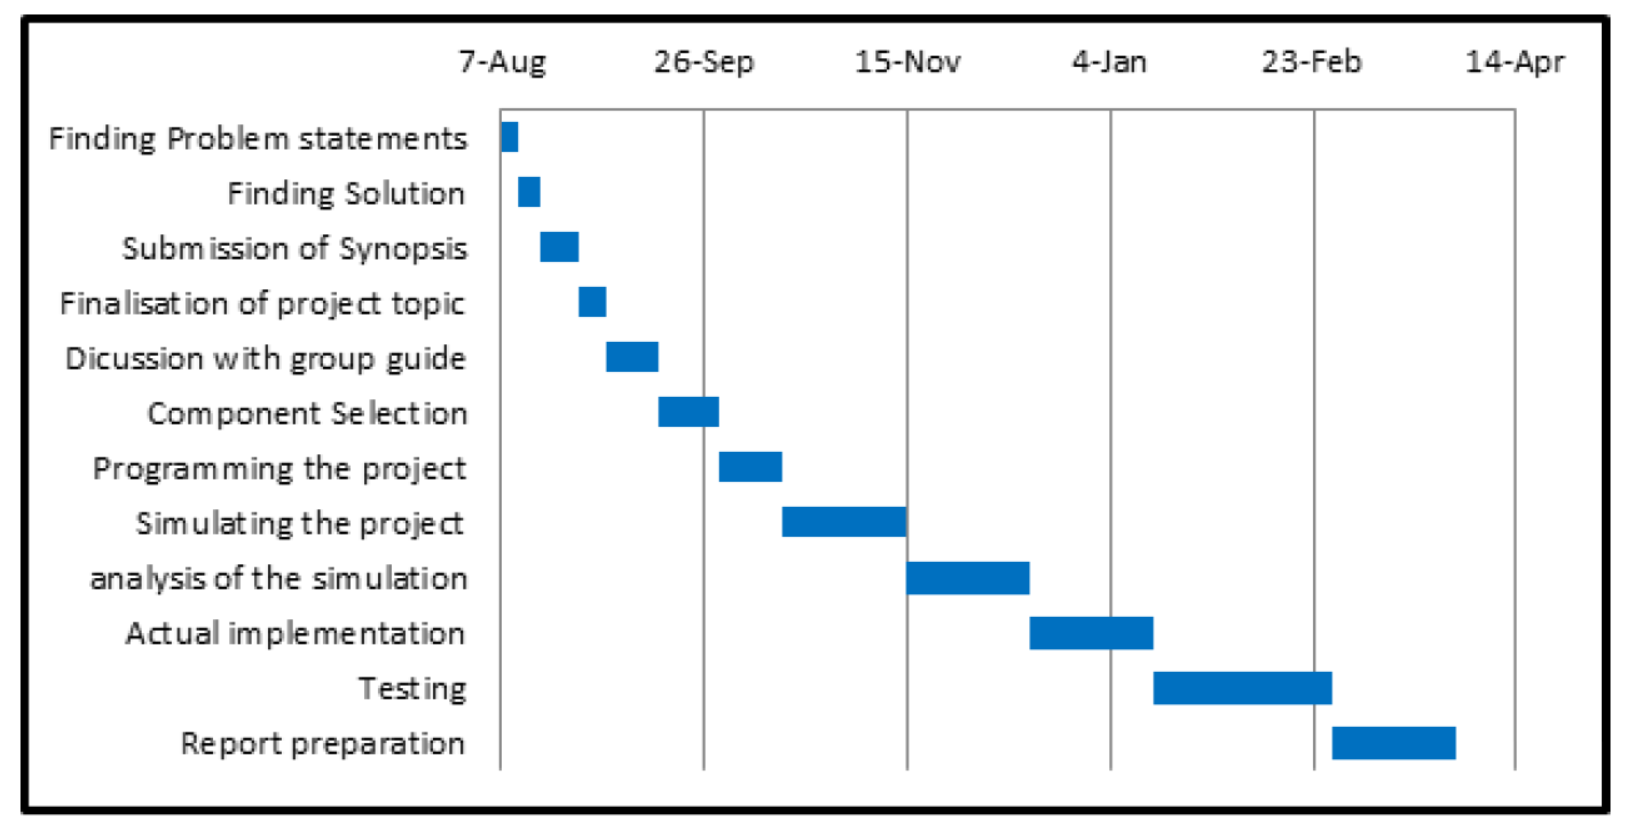
\includegraphics[scale=0.5]{gc.png}\\
\caption{Gantt Chart}
\end{figure}


\newpage
\thispagestyle{empty}
\vspace*{0.25\textheight}
\begin{center}
\begin{center}
{\bfseries\LARGE <------------------------------------------------------<}\\
{\bfseries\LARGE CHAPTER 2}\\[2cm]


{\scshape\Huge LITERATURE SURVEY}
{\bfseries\LARGE <------------------------------------------------------<}
\end{center}
\end{center}

\newpage
\section{LITERATURE SURVEY}

\subsection{Liturature Review}


The Solar Wind Hybrid Electric Vehicle aims to
develop an energy efficient, self-sustaining,
wide-ranging ecofriendly vehicle having a
feature of an automatic switching program to
effectively utilize the power produced by the
solar panel.[1]\\

In the past few years, because of the interest taken in the questions concerning energy consumption and green house effect, renewable energy has become a main concern. Among the different technologies used, wind energy is probably the one which has been developed with the more spectacular increase [1]. Because of their higher efficiency, fast running horizontal axis wind turbines (HAWT) are generally used, but the implementation costs and the necessity to reduce the return-on-investment time have consequently conducted developers to install wind turbine on selected sites where wind velocities are as high as possible. Most of these sites are now equipped and other solutions must be found.\\

Regarding the necessity of using smart grids for energy generation and use, it is clear that local production of electricity has become a necessity, notably on isolated sites and even near or on buildings [2]. In such configurations, not only the delivered power (linked to the efficiency) but also the produced energy must be considered. For example, small turbines running all the time should be preferred to higher ones which only work around nominal running points, generally at a high value of the wind velocity, very rare in such sites.\\

The Savonius rotor [3] or wind turbines derived from this concept are probably interesting solutions which can be found in miscellaneous geometries [4]. Savonius rotors are slow running vertical axis wind turbines (VAWT), i.e. their axis is perpendicular to the incident wind, and their high starting torque permits a running at low wind velocities; finally a main advantage of this is that the behavior does not depend on the wind direction.\\

However, Savonius rotors have two main disadvantages: their efficiency is rather poor and the flow around these machines is very unsteady. These two problems lead to the necessity to correctly predict their aerodynamic performances, which can be done either using numerical simulations (see ref. [5], [6] for example) or using specific experiments. But because of their financial cost, experiments are very difficult to hold and when they are decided, it is generally only for a given geometry. In such a context, an alternative flexible, economical experimental way to assess Savonius rotors is highly desirable.\\

The present study proposes a methodology and an experimental apparatus to predict the aerodynamic performances of slow running VAWTs. The idea is to use very small models (around 10 cm high) which are used in a subsonic wind tunnel. The interest of small models is the ease and speed of manufacture. Testing many models permits to choose the ones which have the most stationary behavior (which is important to minimize mechanical fatigue) and the higher aerodynamic efficiency. However, the use of such small models raises the problem to evaluate a low torque value, in a range where only scarce devices can be found and not totally appropriated to the described objective.\\

To overcome that situation, a mechatronic approach of the problem lead to the development of a simple specific apparatus, which consists in a VAWT linked to a DC motor used as a generator. The characteristics of the motor led to the determination of the mechanical torque on the axis of the turbine and consequently its aerodynamic performances.\\

The present paper presents the methodology to predict the aerodynamics performances of a slow running VAWT using experiments on small models in a specific wind tunnel. In the following the choice of a model is presented, then the apparatus and the experimental protocol are described. Consequently, experimental results are presented and interpreted before we conclude on the concept and the obtained results.\\

A rapid prototyping process was used to fabricate
the small form wind turbine airfoil, a DC motor
was used as a generator to evaluate the generated
power and torque. The aerodynamic performance
of the slow running vertical axis type wind
turbine was evaluated experimentally.[2]\\

Conventional energy sources based on oil, coal, and natural gas have proven to be highly effective drivers of economic progress, but at the same time damaging to the environment and to human health [3]. Nowadays, Renewable energy technologies such as fuel cell and solar are gaining popularity for vehicle application. Not only these energy sources reduce gas in the cities, but they also reduce dependability on the fossil energy [1]. Renewable energies are sources considered as infinite since it can be recycled typically from natural resources found on earth–like solar, wind, and hydro power. Energy saving has been the major pursuit for many who are living in developed cities. In the present day, the most important part of modern living is electricity; we consume electricity to power our homes, offices, and to perform all our daily tasks. Energy conservation has now reached the transportation sector and it has become vital in decreasing the amount of energy we consume. The advent of vehicles with more fuel-efficient engines and the improvement of alternative energy sources have greatly contributed to the conservation of energy.\\

Since Energy consumption and CO2 emission of the road transport are the main issues amongst all impact [5], we develop a vehicle with a renewable source. PV-Wind-Battery-DG hybrid system is the most optimal solution regarding cost and emission among all various hybrid system combinations [2].\\

Furthermore, maximum power point tracking (MPPT) charge controller, instead of the typical PWM-based charge controller, was developed and integrated in the proposed vehicle to attain the maximum power from the solar panel during partial shading at lower and higher solar panel temperature [6]. With the maximum power tracked, a higher current and impedance/load match may be expected.\\

The output power of solar panel that decreased
due to shading has been improved using
bypass diode method. The placement of bypass
diodes increased the output current and power.[3]\\

The need for renewable energy keep increasing [1] by time because the world is running out fossil fuels which were formed millions years ago. If renewable sources are used, the fossil fuels will last longer. The main fossil fuels are oil, natural gas and coal. Oil has some disadvantages such as generating corbon dioxide, causing acid rain and being not clean. Natural gas also has some problems like creating greenhouse gas emmision, being volatile and being dangerous if carelessly transported. Like oil and natural gas, coal creates harmful waste, acid rain and health problem for the miners. The renewable energy is a solution to decrese dependence on fossil energy [2]. There are many sources of renewable energy such as wind, solar and hydroelectricity. Being noisy, being unpredictable and disturbing television and radio signals are three of disadvantages of wind power. Hydroelectricity also has some minuses like disrupting ecosystems, being costly and requiring expensive construction material. Compared to other sources of renewable energy, solar energy is very promising [3] because it is clean [4], cheap, abundant [5], silent [6] and having no pollution.  The solar energy is converted into electrical energy in order to be used in many appliances. A solar cell is an electronic device that use photovoltaic phenomenon to convert sunlight into electrical energy. The smallest building block of solar cell that can generate electricity is called a p-n junction. When packets of energy called photons hit the p-n junction, atoms in, for example, n type region will absorb a photon, so an electron and a hole will be dislodged. After that, a free electron and free hole will be created. These free electrons and holes will later generate current. Mono crystalline, poly crystalline and thin film solar cells are common types of solar cells available in the world. The main material for mono crystalline and poly crystalline solar cells is silicon which is commonly used in the semiconductor industry. Meanwhile, gallium diselenide, amorphous silicon and cadmium telluride  are the common materials which are used to fabricate thin film solar cells. The higher efficiency compared to other type of aolar cells is the main advantage of mono crystalline solar cell. However, due to processes used to enhance the purity, monocrystalline solar cells are expensive compared to other types of solar cells. The highest efficiency of mono crystalline solar cells is around 17 pc-18 pc. There are many factors that can degrade the performance of the solar cell like high temperature, excessive radiation, sand, dust covering the surface of the solar cell and shading. The aim of this work is to improve the performance of solar cells using bypass diodes and blocking diodes.\\

This paper presents a combined experimental
and computational study into the aerodynamics
and performance of a small scale Vertical Axis
Wind Turbine (VAWT)[4].\\

Wind tunnel performance results are presented for cases of different wind velocity, tip-speed ratio and solidity as well as rotor blade surface finish. It is shown experimentally that the surface roughness on the turbine rotor blades has a significant effect on performance. Below a critical wind speed (Reynolds number of 30,000) the performance of the turbine is degraded by a smooth rotor surface finish but above it, the turbine performance is enhanced by a smooth surface finish. Both two bladed and three bladed rotors were tested and a significant increase in performance coefficient is observed for the higher solidity rotors (three bladed rotors) over most of the operating range. Dynamic stalling behaviour and the resulting large and rapid changes in force coefficients and the rotor torque are shown to be the likely cause of changes to rotor pitch angle that occurred during early testing. This small change in pitch angle caused significant decreases in performance.\\

The performance coefficient predicted by the two dimensional computational model is significantly higher than that of the experimental and the three-dimensional CFD model. The predictions show that the presence of the over tip vortices in the 3D simulations is responsible for producing the large difference in efficiency compared to the 2D predictions. The dynamic behaviour of the over tip vortex as a rotor blade rotates through each revolution is also explored in the paper.\\



This paper focuses on a more economical,
noiseless, emission free and uninterrupted
alternate source of electric and hybrid self
charging inverter.[5]\\

Aerosolar vehicles are powered by wind and
sun/solar energy.[6]

Wind energy, solar energy, dynamo motors,
solar array, alternators, DC motor.\\

\newpage
\thispagestyle{empty}
\vspace*{0.25\textheight}
\begin{center}
\begin{center}
{\bfseries\LARGE <------------------------------------------------------<}\\
{\bfseries\LARGE CHAPTER 3}\\[2cm]


{\scshape\Huge DESIGN METHODOLOGY}
{\bfseries\LARGE <------------------------------------------------------<}
\end{center}
\end{center}
\newpage
\section{DESIGN METHODOLOGY}
\subsection{System Requirements and Specifications}

\textbf{Solar Panel - 10 Watt}\\[1cm]
This 10W solar panel is rigid with a metal frame. Superior durability over flexible panels. Great for portable or permanent installations. Can be used to charge any 12V battery, for example, those powering electric fence energizers, camping, recharging automotive batteries, etc. The panel can be purchased with a charge controller so it is safe for use in charging 12V batteries.\\
\textbf{Specification}
\begin{itemize}
\item Performance : Best in Class Efficiency {10.03p.c}, Innovative cell technology ensures optimum solarpower generation providing high value for money upto16.5p.c.
\item Enhanced Performance : Low - Light Performance, After 25 years, Loom Solar 10W is guaranteed at least 80% of initial performance.
\item Application : Perfect for charging Power Bank/Mobile/Small Battery upto 20AH
\item Technology : Poly Crystalline Technology, PID Resistance Technology
\item Dimension : (L*W*H) mm 285 x 350 x 22mm

\end{itemize}
\begin{figure}[!h]
\centering
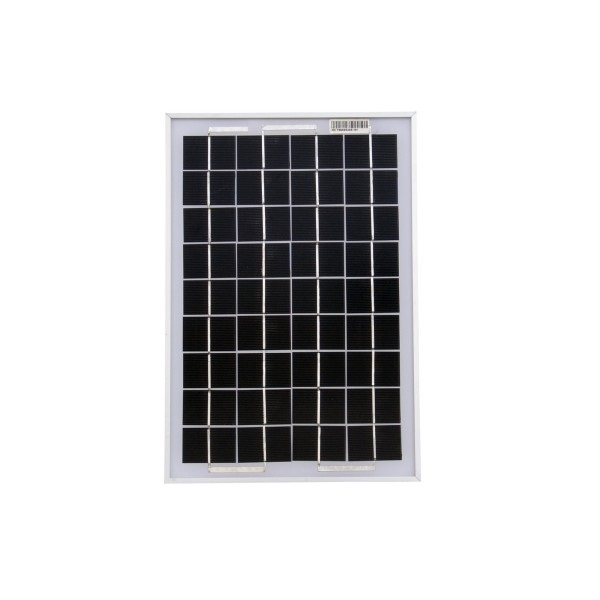
\includegraphics[scale=0.4]{sp.jpg}\\
\caption{Solar Panel 10W}
\end{figure}

\newpage
\textbf{Wind Turbine – 3 blades Vertical Axis}\\[1cm]
\textbf{Specification}
\begin{itemize}
\item Material: Plastic+Electrical components
\item Color: White and Pink
\item Output voltage : DC 0.01v - 5.5v
\item Output current : 0.01 - 100mA
\item Rated speed : 100 - 6000 rev/min
\item Motor diameter : 24.5mm/0.96"(appr.)
\item Motor height : 34.2mm/1.35"(appr.)
\item Motor shaft diameter : 2mm/0.079"(appr.)
\item Motor shaft length : 13.5mm/0.53"(appr.)
\item Blade Size: (Dia.)X(H)10*7cm(after assembling)
\end{itemize}
\begin{figure}[!h]
\centering
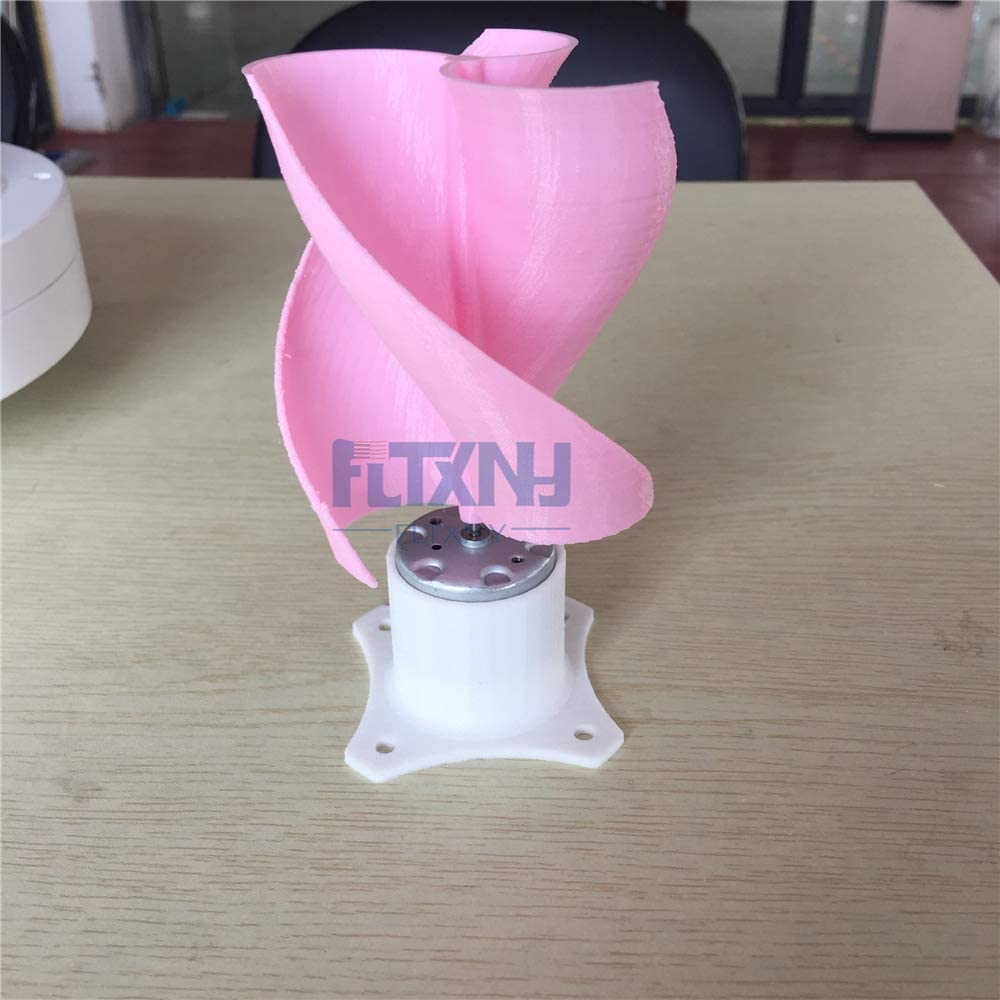
\includegraphics[scale=0.2]{wt.jpg}\\
\caption{Vertical Axis Wind Turbine}
\end{figure}

\textbf{DC Motor}\\[1cm]
The 6V 250mA Brushed DC Motor is a standard '130 size' DC hobby motor. It comes with a wider
operating range than most toy motors: from 4.5 to 9VDC instead of 1.5-4.5V. This range makes them
perfect for controlling with an Adafruit Motor Shield, or with an Arduino where you are more likely to
have 5 or 9V available than a high current 3V setting. It will fit in most electronics that already have
130-size motors installed and there's two breadboard-friendly wires soldered on already for fast
prototyping\\
\begin{figure}[!h]
\centering
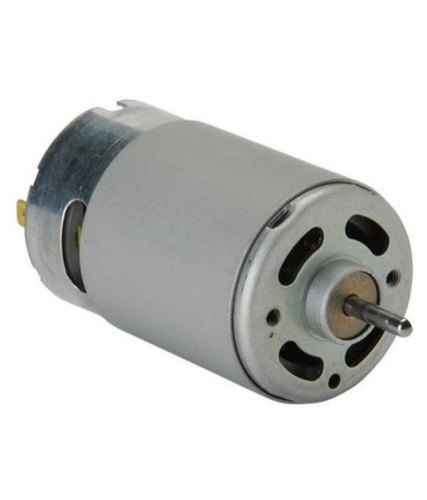
\includegraphics[scale=0.3]{dc.jpeg}\\
\caption{DC Motor 6v}
\end{figure}

\textbf{Microcontroller – PIC18F4550}\\[1cm]
This family of devices offers the advantages of all
PIC18 microcontrollers – namely, high computational
performance at an economical price – with the addition
of high endurance, Enhanced Flash program memory. In addition to these features, the
PIC18F2455/2550/4455/4550 family introduces design
enhancements that make these microcontrollers a logical choice for many high-performance, power sensitive
applications\\
\begin{figure}[!h]
\centering
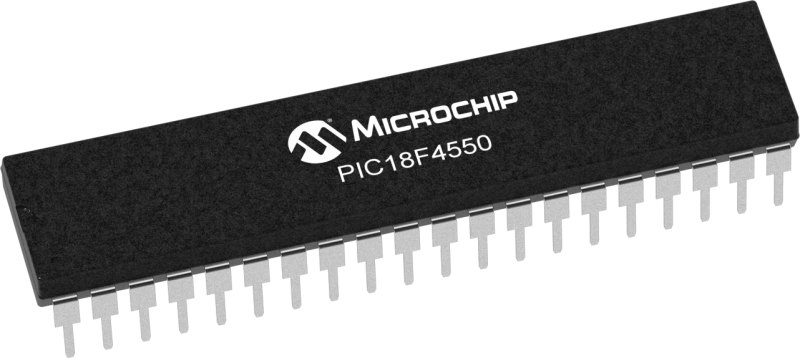
\includegraphics[scale=0.3]{uc.jpg}\\
\caption{Microcontroller PIC18F4550}
\end{figure}

\textbf{BLDC Motor}\\[1cm]
A motor converts supplied electrical energy into mechanical energy. Various types of motors are in common use. Among these, brushless DC motors (BLDC) feature high efficiency and excellent controllability, and are widely used in many applications. The BLDC motor has power-saving advantages relative to other motor types.\\
\textbf{Specification}
\begin{itemize}
\item Frame size: 23 Frame
\item Power (watt) 60W
\item Current (Amp) 3A to 6A
\item Torque 0.3 to 0.8 Nm
\item Voltage range ±Variation (± 10pc) 12V or 24V or 48 V
\item Speed (RPM) 1500 or 3000
\item Motor poles 4Pole
\item Hall Sensor Yes 3 hall sensors
\item Mounting Flange
\item Degree of protection IP 44
\item Class of insulation F
\item Ambient Temp. / Max Temp. 50° C / 70° C
\item Duty / Rating S1/ continuous
\item Direction of rotation Bi-directional
\item Cooling Naturally Ventilated
\item Shaft 12 Dia X 29 mm L
\item Motor 65 mm diameter X 65 mm Length
\end{itemize}

\begin{figure}[!h]
\centering
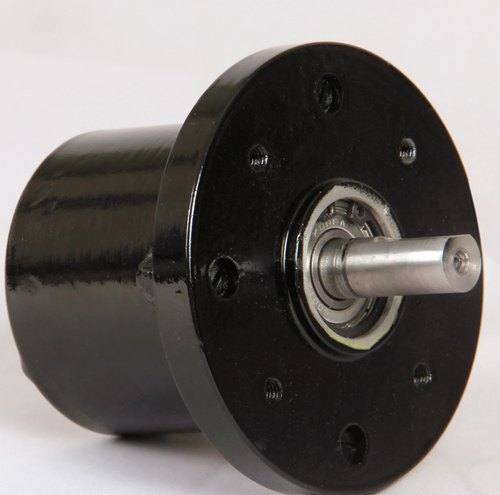
\includegraphics[scale=0.25]{bldc.jpg}\\
\caption{BLDC Motor 60W}
\end{figure}

\textbf{Battery}\\[1cm]
A lithium-ion battery is a family of rechargeable battery types in
which lithium ions move from the negative electrode to the positive
electrode during discharge and back when charging. Lithium-ion
batteries are common in consumer electronics. They are one of the
most popular types of rechargeable battery for portable electronics, with one of the best energy-to-weight ratios, high open circuit
voltage, low self-discharge rate, no memory effect and a slow loss of
charge when not in use.\\
\textbf{Specification}
\begin{itemize}
\item Voltage: 12 Volt
\item Battery Type: Lithium-Ion or Dry-Cell
\item Capacity: 2.5Ah
\end{itemize}

\begin{figure}[!h]
\centering
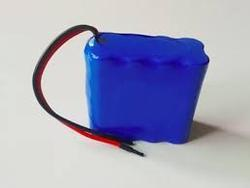
\includegraphics[scale=0.75]{b.jpg}\\
\caption{Lithium-Ion Battery 12v, 2.5Ah}
\end{figure}
\textbf{LM3914}\\[1cm]
The simplified LM3914 block diagram is to give the general idea of the circuit's operation. A high input
impedance buffer operates with signals from ground to 12V, and is protected against reverse and overvoltage
signals. The signal is then applied to a series of 10 comparators; each of which is biased to a different
comparison level by the resistor string.\\
In the example illustrated, the resistor string is connected to the internal 1.25V reference voltage. In this case, for
each 125mV that the input signal increases, a comparator will switch on another indicating LED. This resistor
divider can be connected between any 2 voltages, providing that they are 1.5V below Vplus and no less than Vminus If
an expanded scale meter display is desired, the total divider voltage can be as little as 200mV. Expanded-scale
meter displays are more accurate and the segments light uniformly only if bar mode is used. At 50mV or more
per step, dot mode is usable.\\

\begin{figure}[!h]
\centering
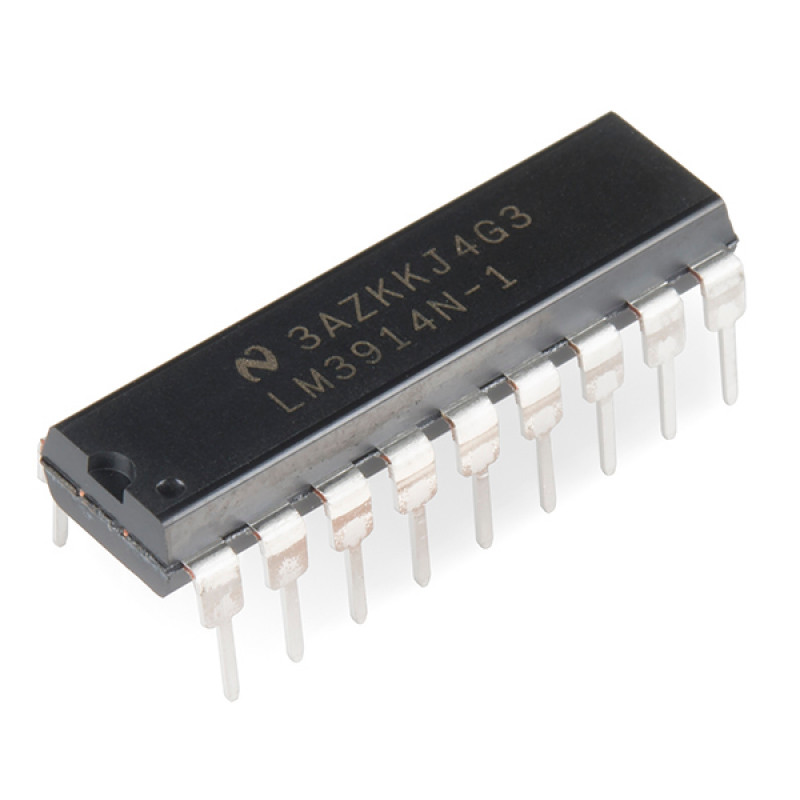
\includegraphics[scale=0.3]{lm3914.jpg}\\
\caption{LM3914 IC}
\end{figure}

\textbf{Buck Converter}\\[1cm]
The TPS40222 is a fixed-frequency, current-mode,
non-synchronous buck converter optimized for
applications powered by a 5-V distributed source.
With internally determined operating frequency,
soft-start time, and control loop compensation, the
TPS40222 provides many features with a minimum of
external components.\\
The TPS40222 operates at 1.25 MHz and supports
up to 1.6-A output loads. The output voltage can be
programmed to as low as 0.8 V. The TPS40222
utilizes pulse-by-pulse current limit as well as
frequency foldback to protect the converter during a
catastrophic short circuited output condition.\\

\begin{figure}[!h]
\centering
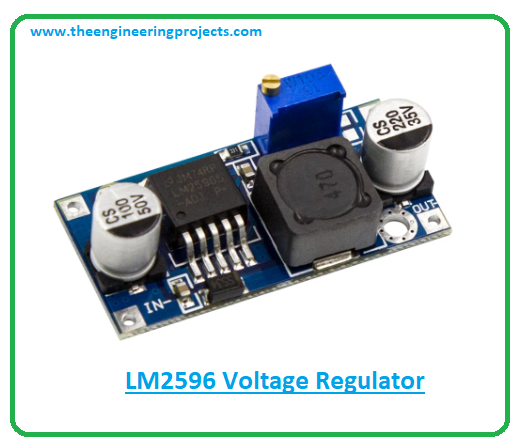
\includegraphics[scale=0.5]{bc.png}\\
\caption{Buck Converter}
\end{figure}

\newpage
\subsection{Block Diagram and Description}.
  \\[6cm]
\begin{figure}[!h]
\centering
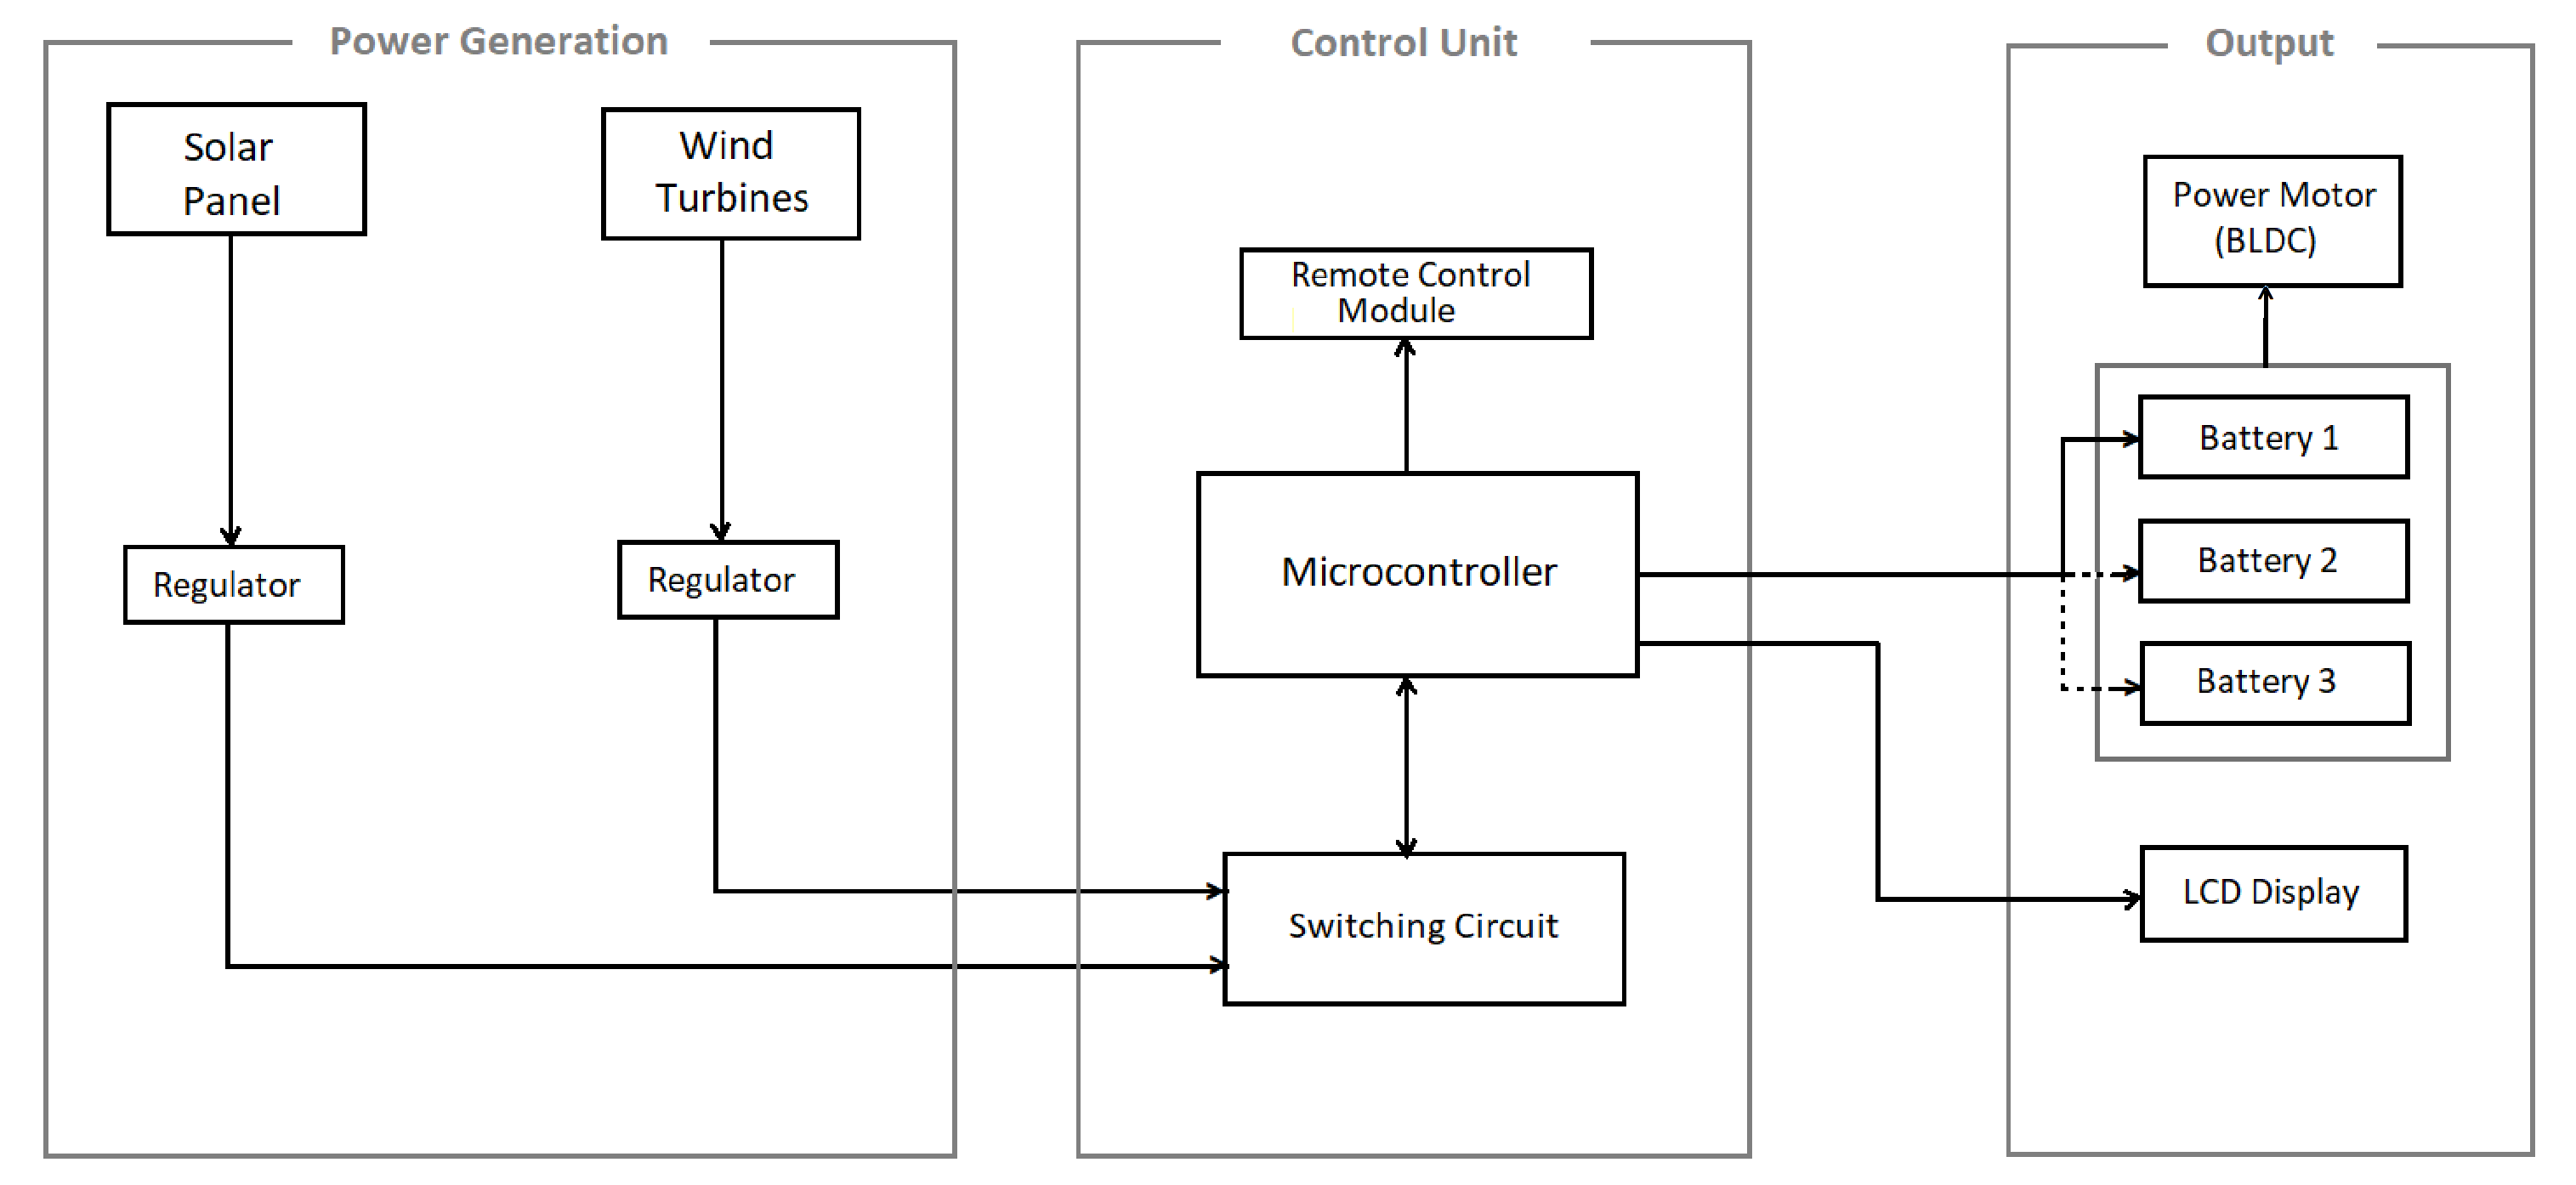
\includegraphics[scale=0.2]{bd.png}\\
\caption{. Block diagram}
\end{figure}

\newpage
\textbf{Block Discription}\\[1cm]
The block diagram mainly consists of three blocks:-
\begin{itemize}
\item Power Generation Block
\item Control Block
\item Output Block
\end{itemize}
\subsubsection{Power Generation Block}
It consist of solar panel and vertical wind turbine as power generation. The regulators are used to regulate the voltage generated by both. The solar panel generates more power as compared to wind turbine. Hence solar panel recharges the battery at higher rate than wind turbine.

\subsubsection{Control Block}
This block contains remote control module, microcontroller and overcharging avoiding circuit. The remote control module is used to move the vehicle wirelessly. Microcontroller PIC24 is the heart of the vehicle, which controls the charging of the batteries. The overcharging avoiding circuit saves the battery from overcharging.

\subsubsection{Output Block}
The output block contains power motor(BLDC), battery and LCD display. The BLDC motor is used to drive the vehicle. The battery block has 3 batteries of same specifications. To connect a battery with the motor we used rotative switching technique. LCD displays the battery percentage.

\newpage
\subsection{Hardware Design}
\textbf{Hardware}\\[1cm]
\begin{figure}[!h]
\centering
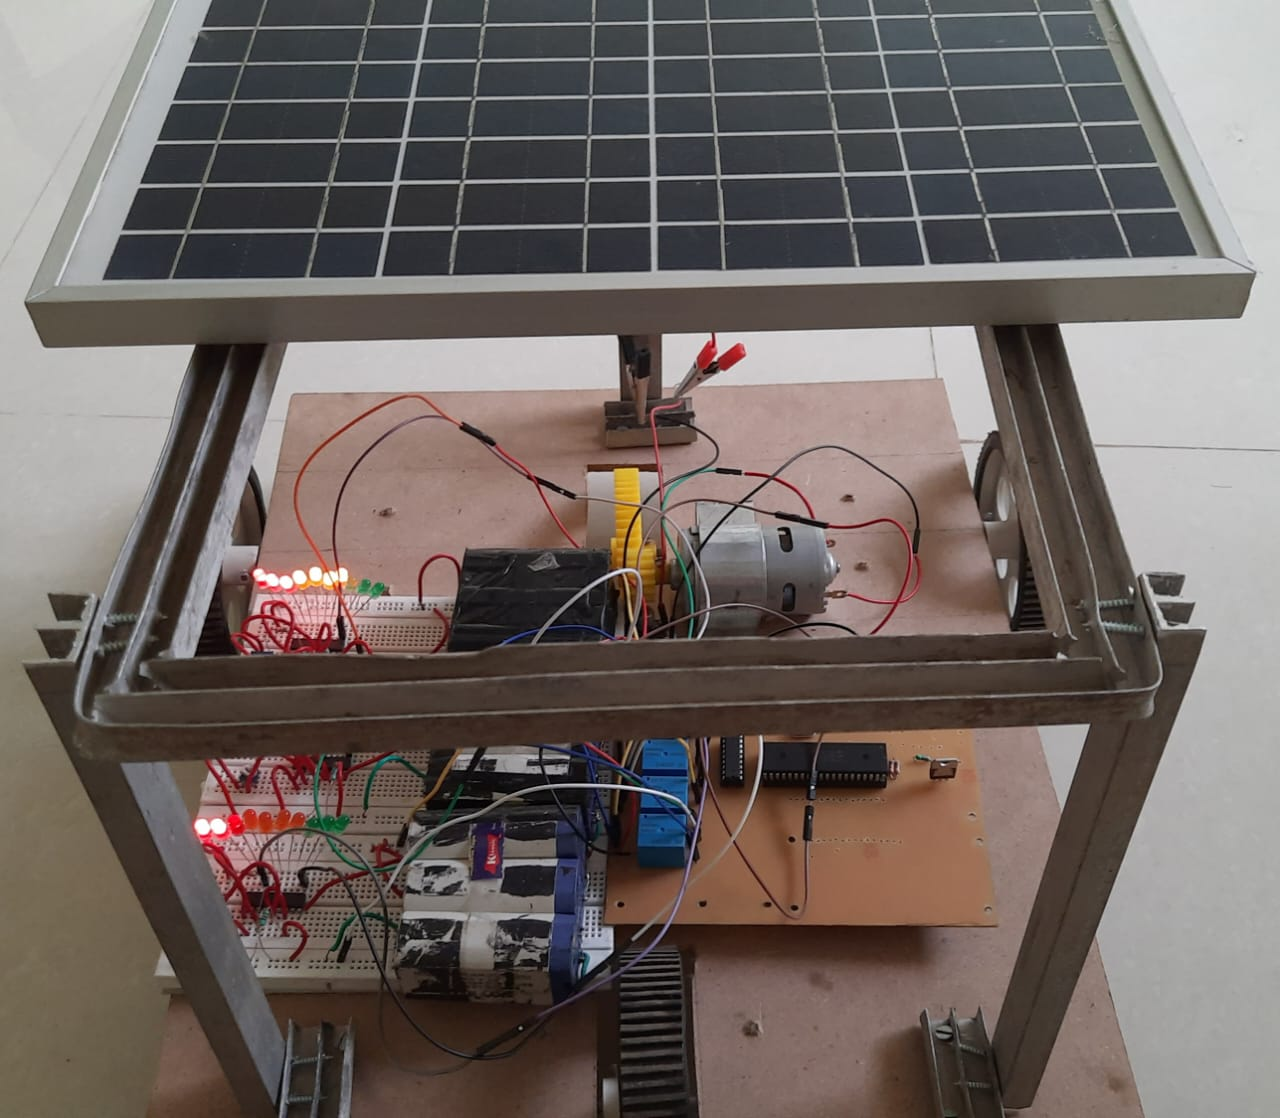
\includegraphics[scale=0.3]{hw1.jpeg}\\
\caption{. Hardware}
\end{figure}\\
The above image show the hardware circuit of the project. Here three batteries are connected to switching circuit and are powering the motor. Also the discharged batteries are charged.\\
This 10W solar panel is rigid with a metal frame. Superior durability over flexible panels. Great for portable or permanent installations. Can be used to charge any 12V battery, for example, those powering electric fence energizers, camping, recharging automotive batteries, etc. The panel can be purchased with a charge controller so it is safe for use in charging 12V batteries.

\newpage
\textbf{Front View of EV}\\[1cm]
\begin{figure}[!h]
\centering
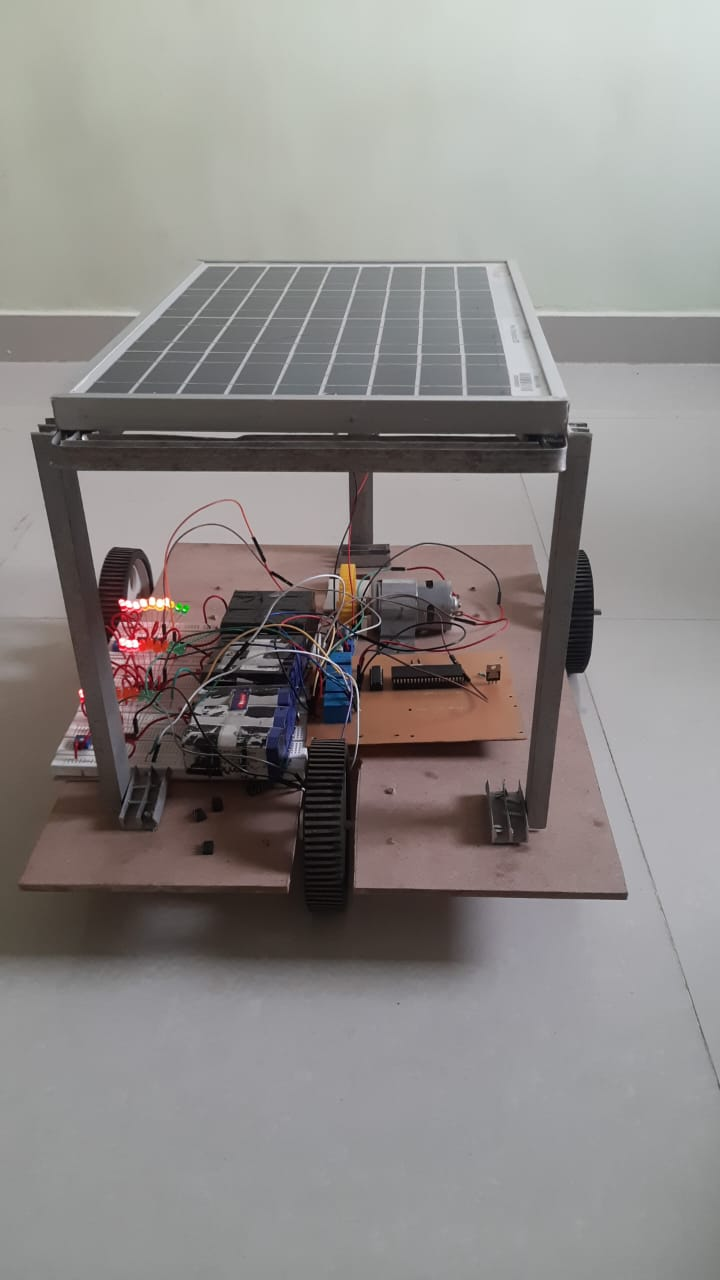
\includegraphics[scale=0.3]{fv.jpeg}\\
\caption{. Front View of EV}
\end{figure}

The above figure shows the front view of the electric vehicle.\\
A motor converts supplied electrical energy into mechanical energy. Various types of motors are in common use. Among these, brushless DC motors (BLDC) feature high efficiency and excellent controllability, and are widely used in many applications. The BLDC motor has power-saving advantages relative to other motor types.

\newpage
\textbf{Side View of EV}\\[1cm]
\begin{figure}[!h]
\centering
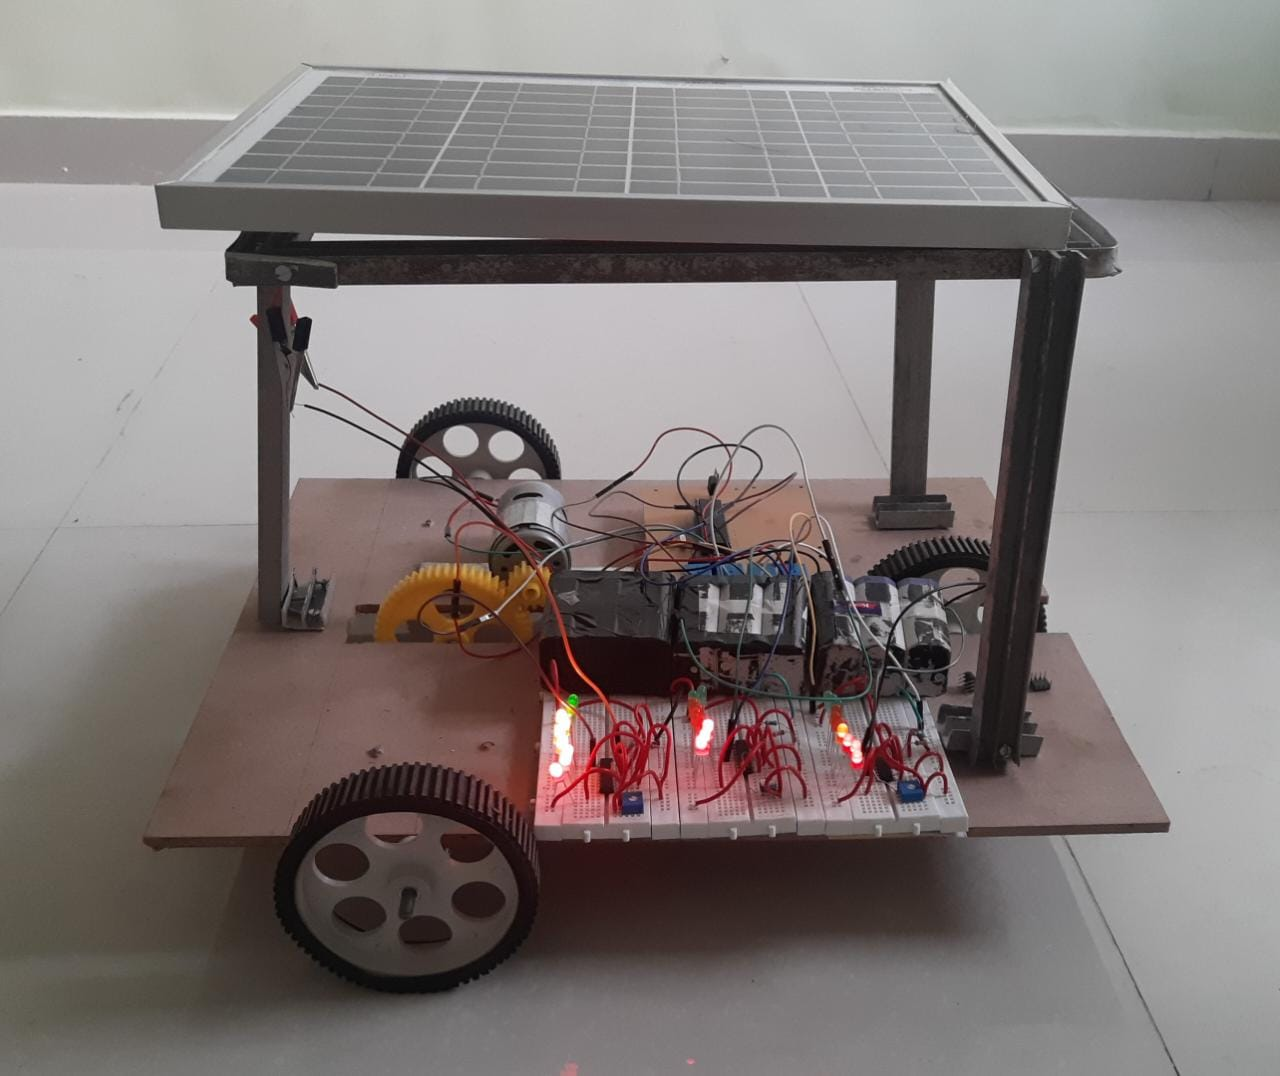
\includegraphics[scale=0.3]{sv.jpeg}\\
\caption{. Side View of EV}
\end{figure}

The above figure shows the side view of the electric vehicle.\\[1cm]
\textbf{Calculations}\\[0.5cm]
Mass of the vehicle=20Kg\\
Max. Velocity= 10m/s\\
Total force required for the vehicle F=6N\\
Total Power required P=F x V= 6 x 10= 60Watt\\
Therefore, the required battery is of 12V x 2.5A= 60Watt

\newpage
\subsection{Methodology}
\begin{itemize}
\item Solar panel and wind turbine are used for charging the batteries with voltage
regulators and rectifiers.

\item Over charging of the batteries is avoided with the help of microcontroller and over
charging avoiding circuit.

\item The power motor gets a sufficient power from batteries using microcontroller for
driving the vehicle.

\item Remote controlled module is used for performing the movement of the vehicle.

\item The LCD display will show the percentage of battery.

\item Microcontroller will switch between the batteries according to their remaining
percentages with the help of rotative switching technique.

\item The rotative switching technique works with simple trick. Initially the BLDC motor is powered by 'Battery1'. When it discharges upto 40 percent, then the power from 'Battery1' is switched to 'Battery2' and the 'Battery1' starts charging from solar panel. The same process happens when 'Battery2' is discharged, but here solar panel charges 'Battery2' and 'Battery1' is charged with wind turbine. This process continues until the average percentage of all batteries come upto 10 percent.

\item As the battery percentage is below 10 percent, it will initiate the alarm.
\end{itemize}

\newpage
\subsection{Software Design}

\begin{figure}[!h]
\centering
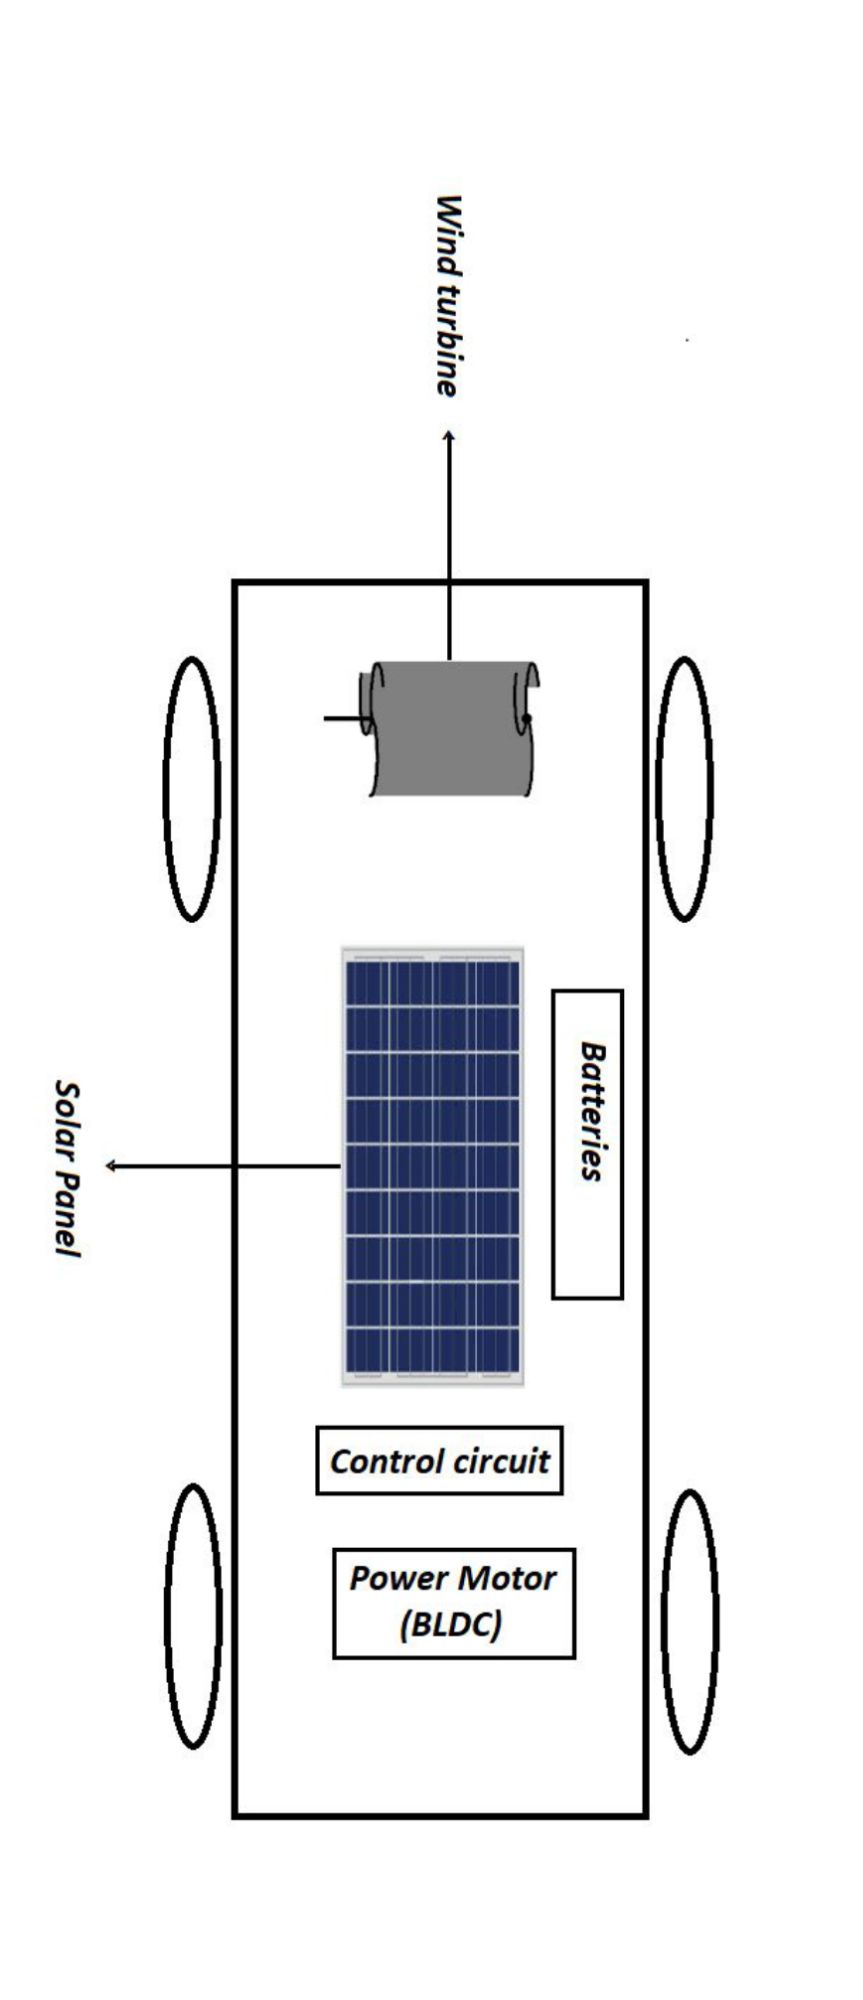
\includegraphics[scale=0.25]{di.jpg}\\
\caption{. Schematic Design}
\end{figure}
Figure 3.5.14 shows the annimated top view of the EV.\\

\newpage
\subsubsection{Modern Tools Used}
\begin{figure}[!h]
\centering
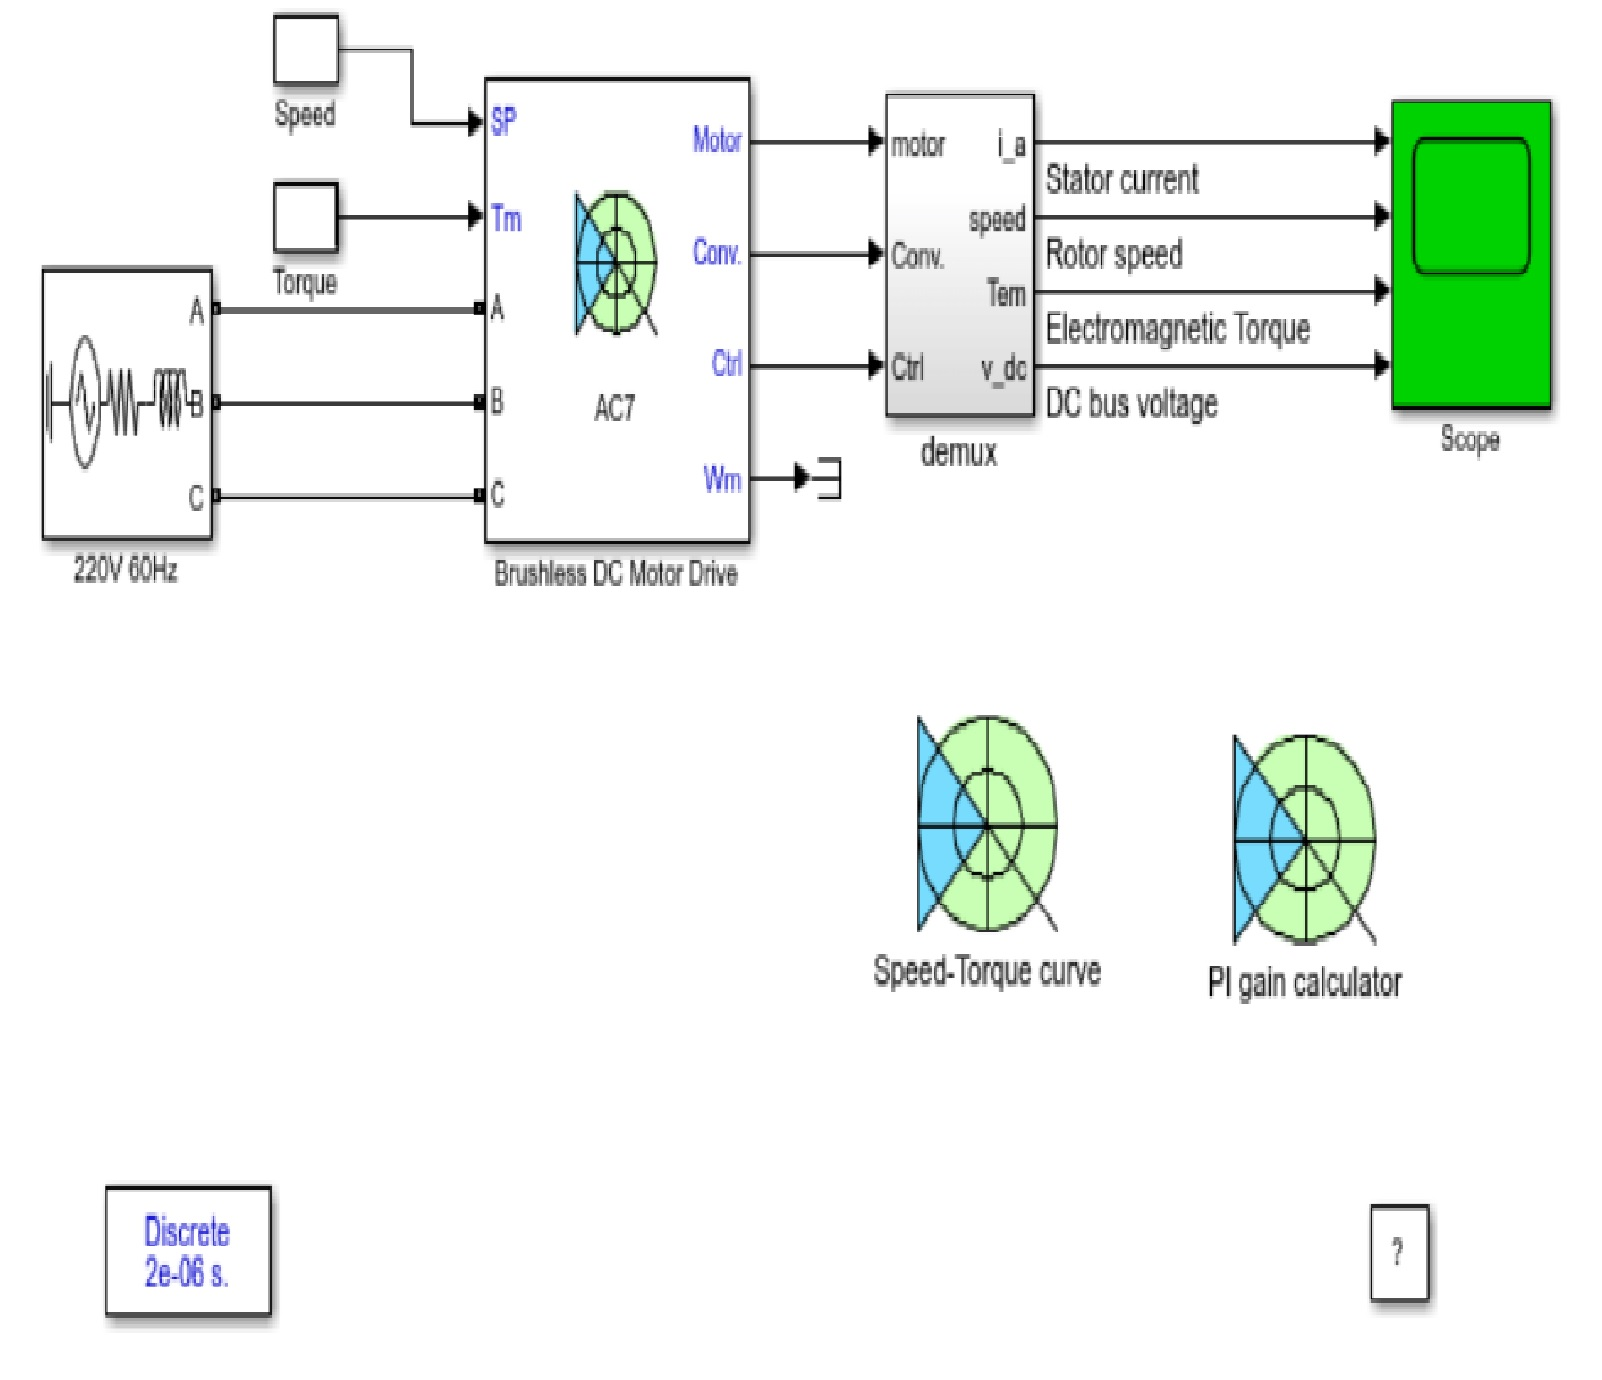
\includegraphics[scale=0.3]{bl.jpg}\\
\caption{. Brushless DC Motor Drive During Speed Regulation}
\end{figure}
Figure 3.5.15 shows the simulation of BLDC motor driving in simulink.\\

\begin{figure}[!h]
\centering
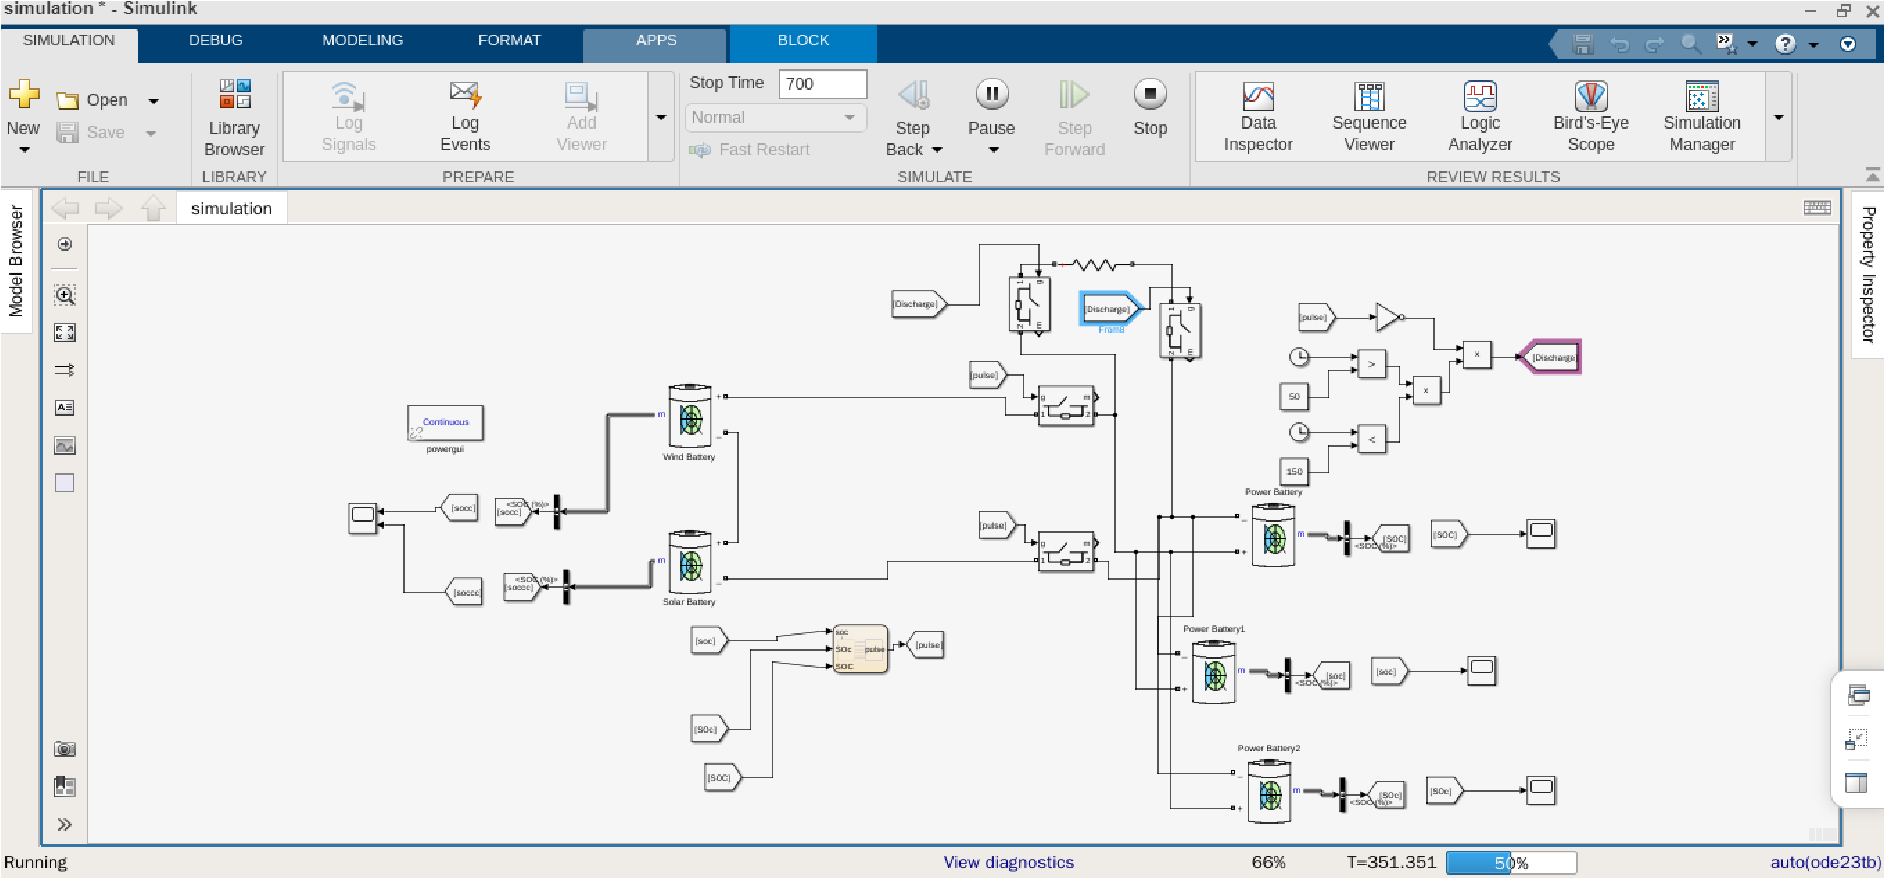
\includegraphics[scale=0.3]{Sim.png}\\
\caption{. Matlab Simulation}
\end{figure}
Figure 3.5.16 shows the simultaion of switching circuit in simulink.\\

\newpage
\begin{figure}[!h]
\centering
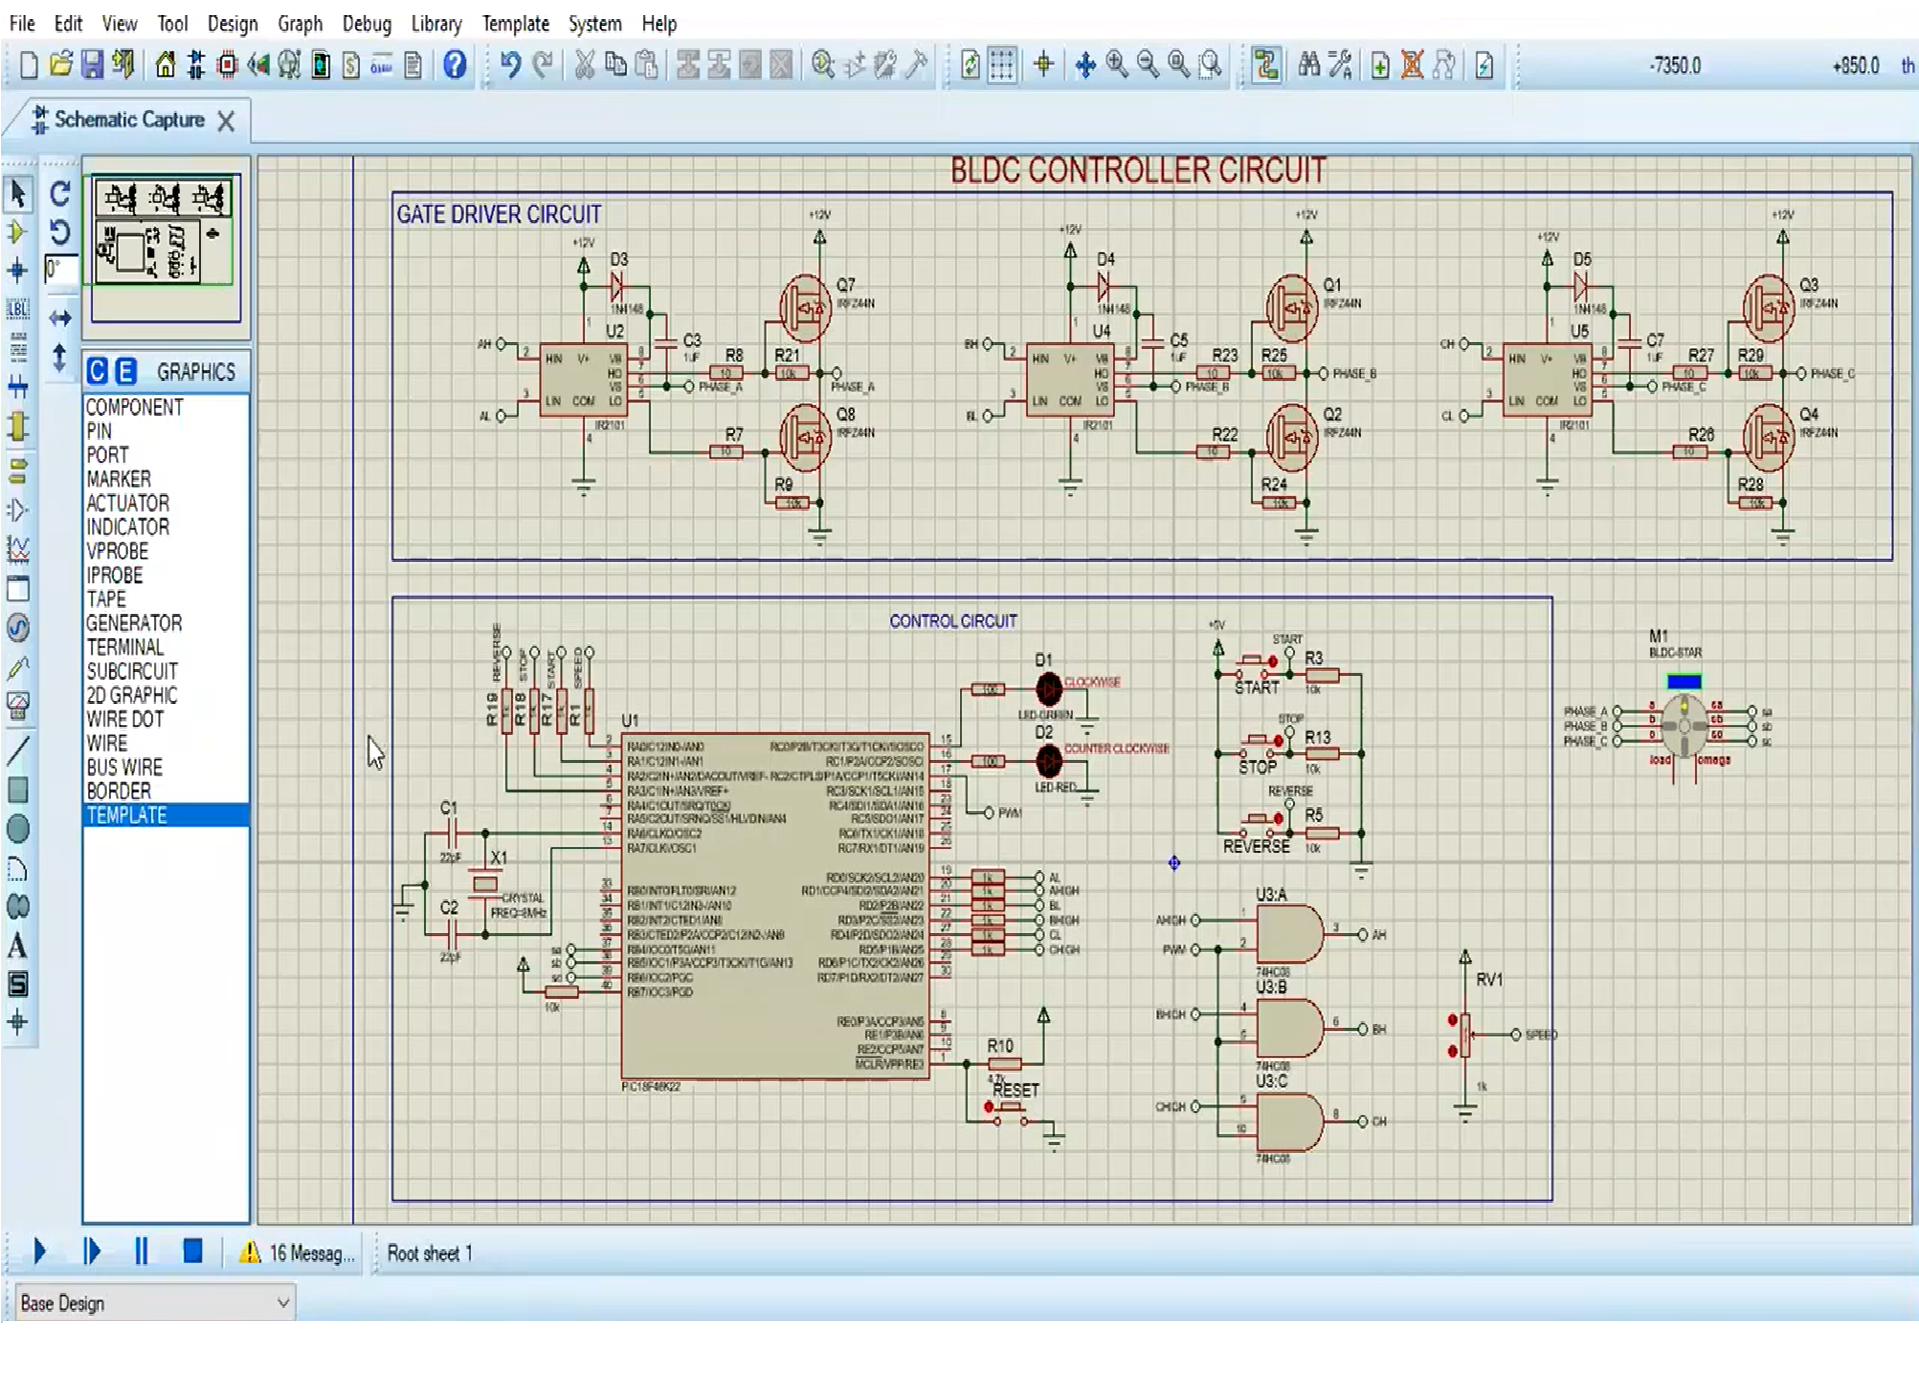
\includegraphics[scale=0.3]{ckt.png}\\
\caption{. BLDC Motor Driver Circuit}
\end{figure}
Figure 3.5.17 shows the BLDC motor driver circuit in proteus.\\

\begin{figure}[!h]
\centering
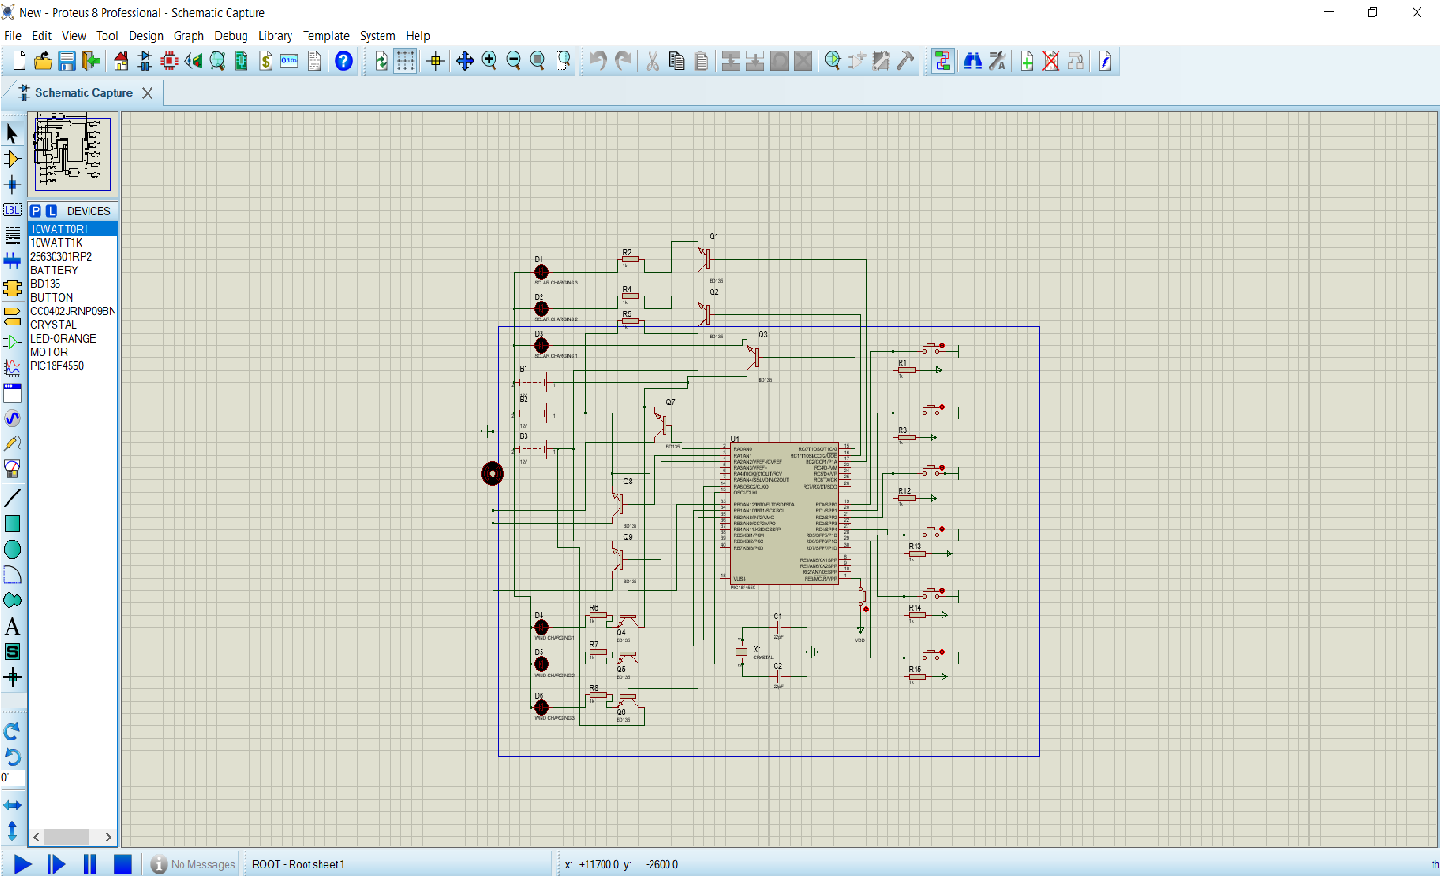
\includegraphics[scale=0.5]{swckt.png}\\
\caption{. Switching Circuit}
\end{figure}
Figure 3.5.18 shows the switching circuit in the proteus. This shows the solar charging battery, wind charging battery and the discharging battery, and also switches between them according to their battery percentage.\\

\newpage
\begin{figure}[!h]
\centering
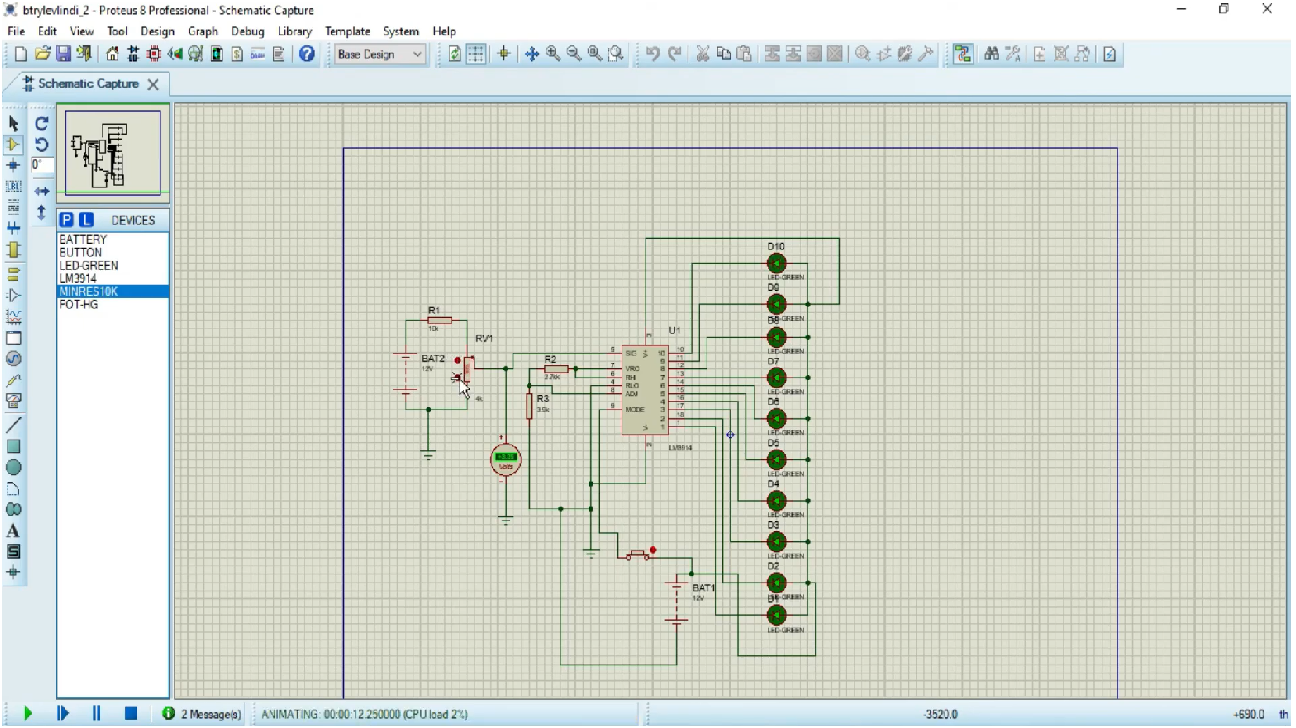
\includegraphics[scale=0.5]{bli.png}\\
\caption{. Battery Level Indicator Circuit}
\end{figure}
Figure 3.5.19 shows the battery level indicator. It shows how much charge percentage is remaining in the battery. It has 10 LEDs that show 10percent battery each.\\

\newpage
\subsection{PCB}

\begin{figure}[!h]
\centering
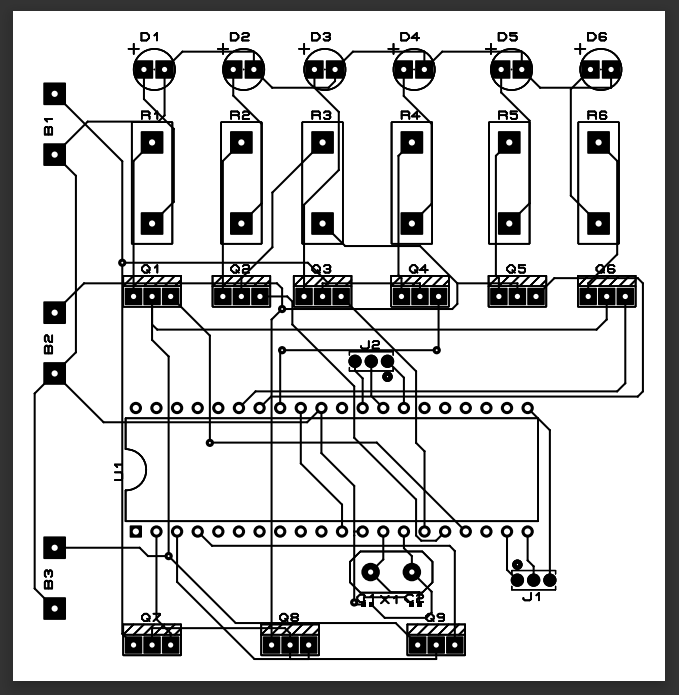
\includegraphics[scale=0.5]{pcbl.png}\\
\caption{. PCB Layout}
\end{figure}

\begin{figure}[!h]
\centering
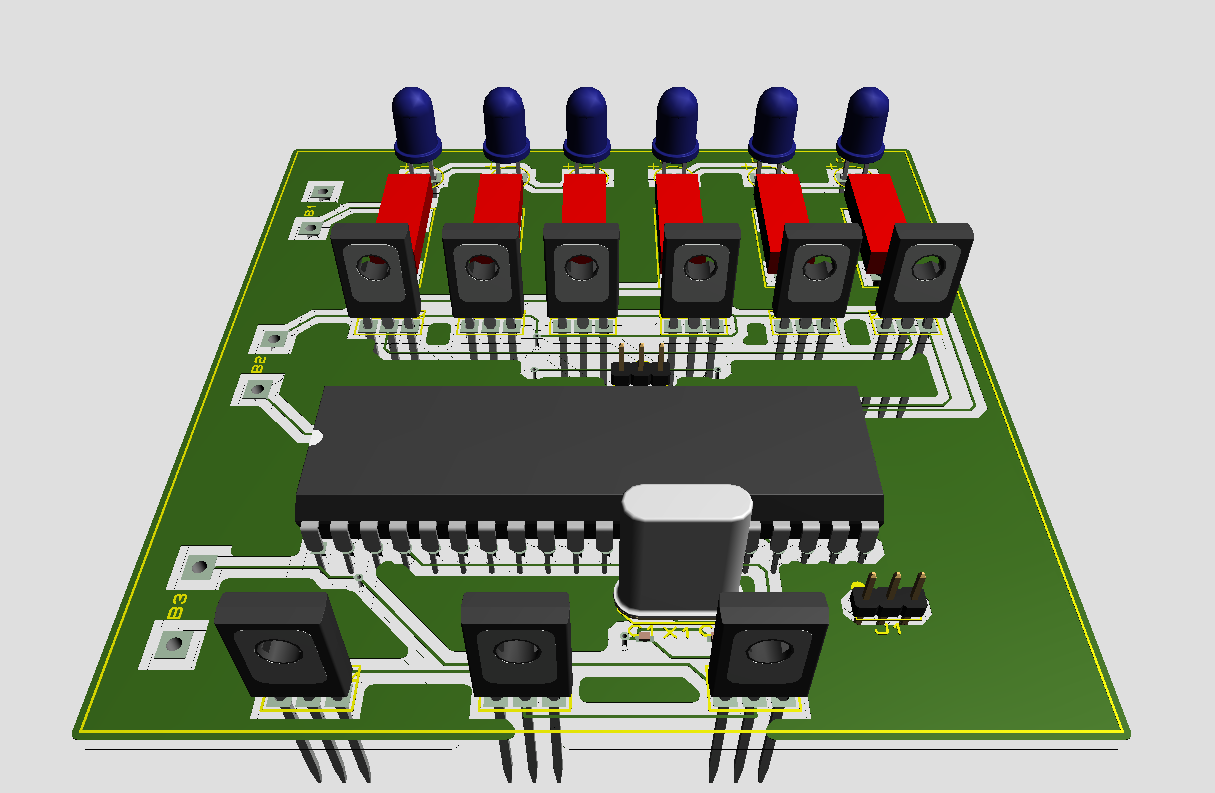
\includegraphics[scale=0.5]{3dpcb.png}\\
\caption{. 3D view PCB}
\end{figure}

\newpage

\newpage
\newpage
\thispagestyle{empty}
\vspace*{0.25\textheight}
\begin{center}
\begin{center}
{\bfseries\LARGE <------------------------------------------------------<}\\
{\bfseries\LARGE CHAPTER 4}\\[2cm]


{\scshape\Huge TEST PROCEDURES AND}\\[0.5cm]
{\scshape\Huge AND}\\[0.5cm]
{\scshape\Huge RESULTS}
{\bfseries\LARGE <------------------------------------------------------<}
\end{center}
\end{center}
\newpage
\section{Test Procedure and Results}
\subsection{Simulation Results}
\begin{figure}[!h]
\centering
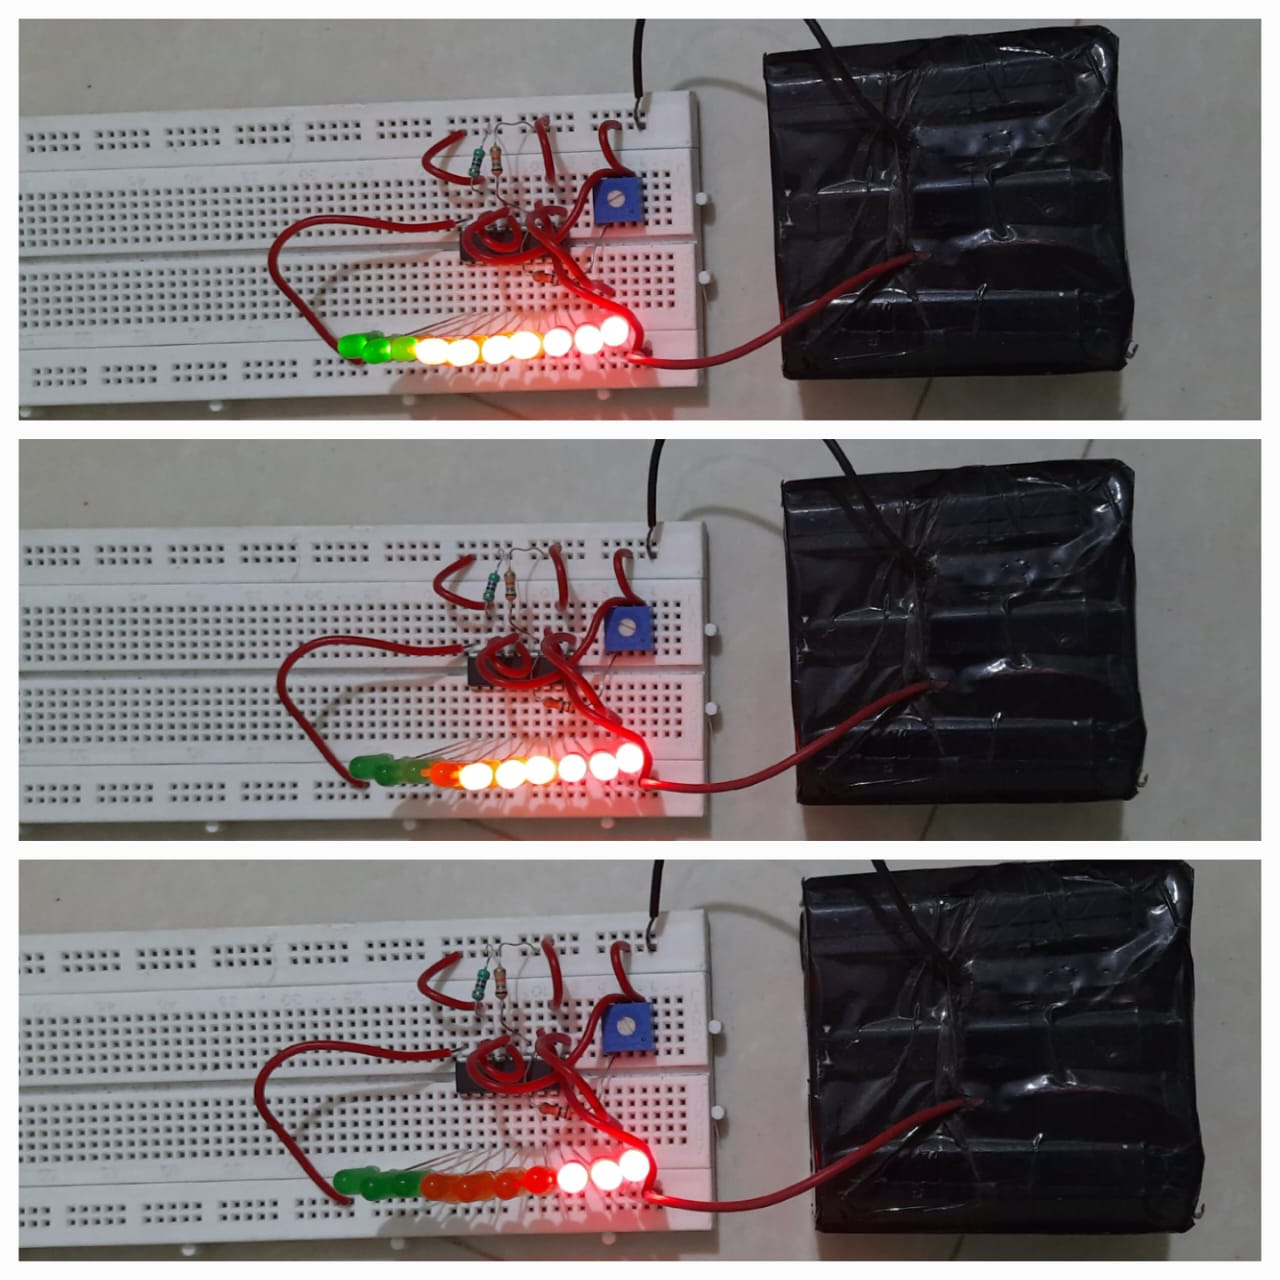
\includegraphics[scale=0.3]{bli.jpeg}\\
\caption{. Battery Level Indicator}
\end{figure}

The image shows the battery level indicator. Each LED shows 10pc charge. First image shows 100 pc battery charged. Second image shows 60 pc battery charged. Third image shows 30 pc battery charged. \\

\newpage
\begin{figure}[!h]
\centering
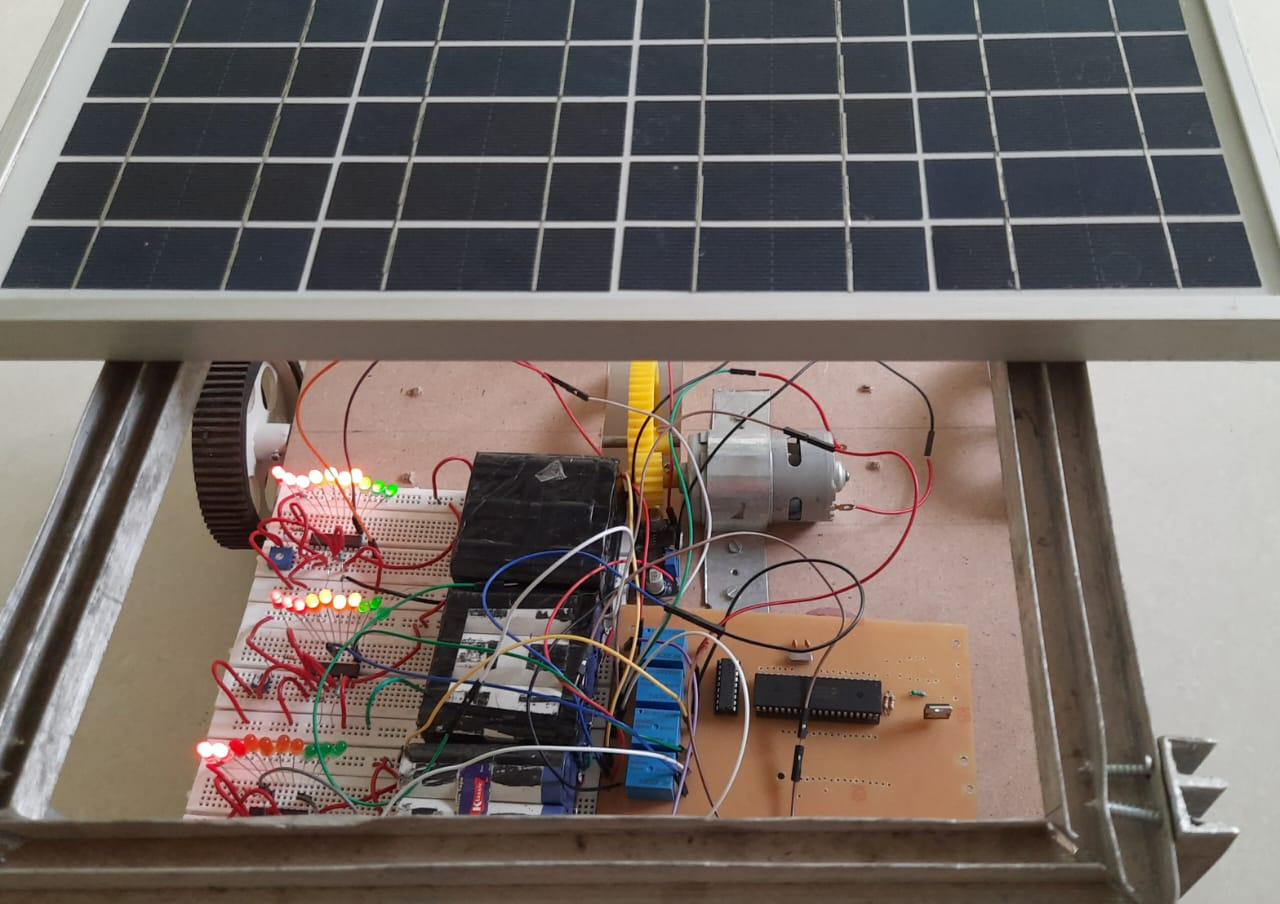
\includegraphics[scale=0.25]{hw2.jpeg}\\
\caption{. Test Stage1}
\end{figure}

Here 1st battery is discharged and it has started charging. And 2nd battery started discharging.\\

\begin{figure}[!h]
\centering
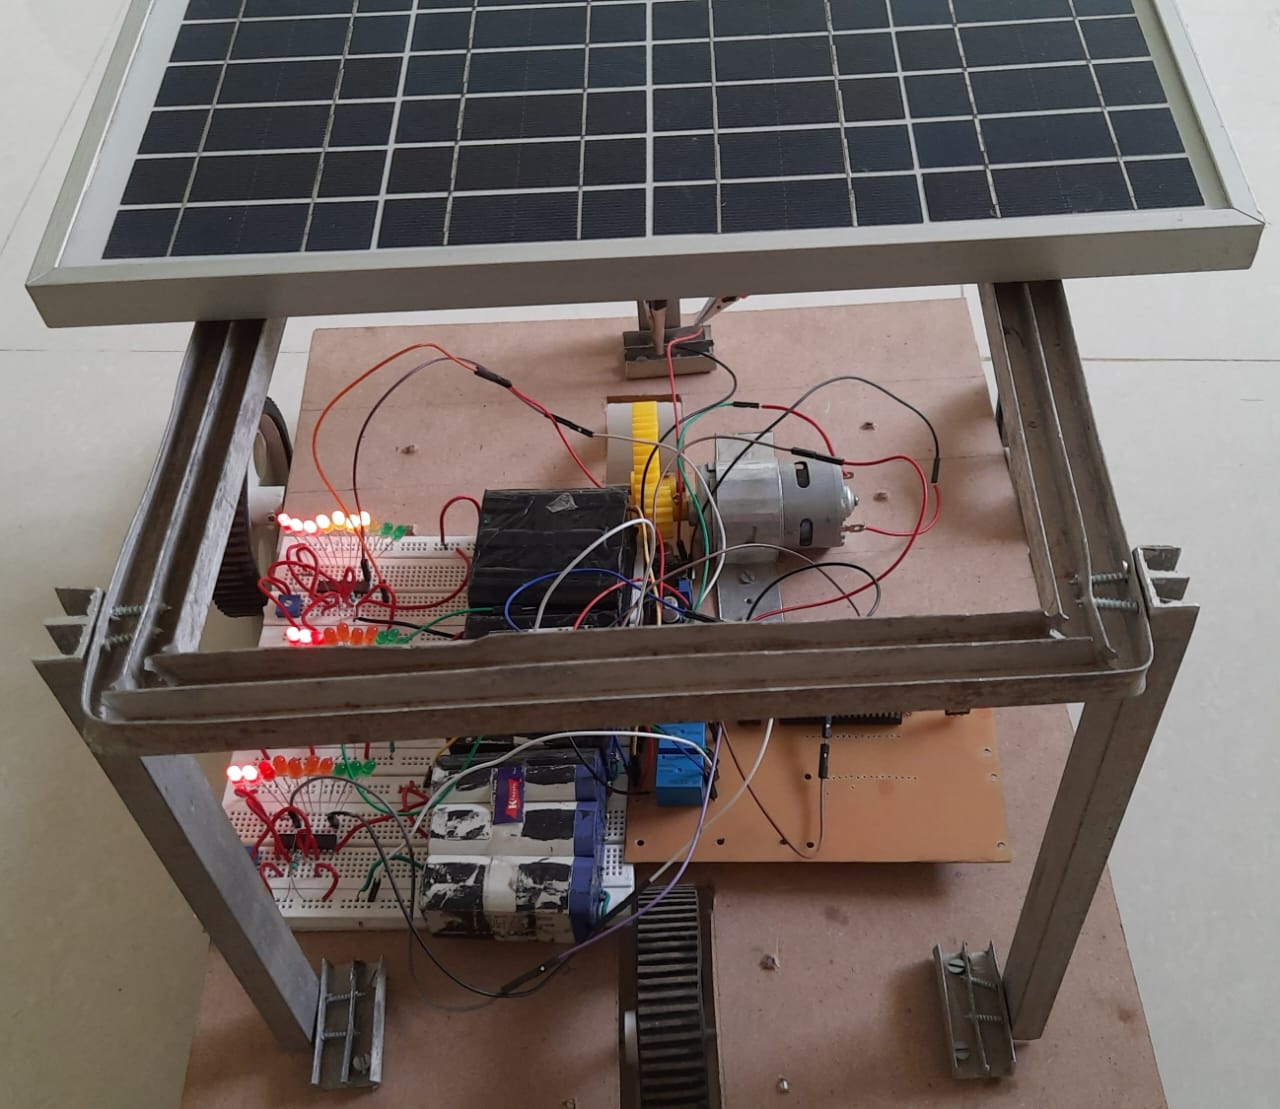
\includegraphics[scale=0.25]{hw3.jpeg}\\
\caption{. Test Stage2}
\end{figure}

Here 2nd battery is discharged and it has started charging. And 3rd battery started discharging.\\

\newpage
\begin{figure}[!h]
\centering
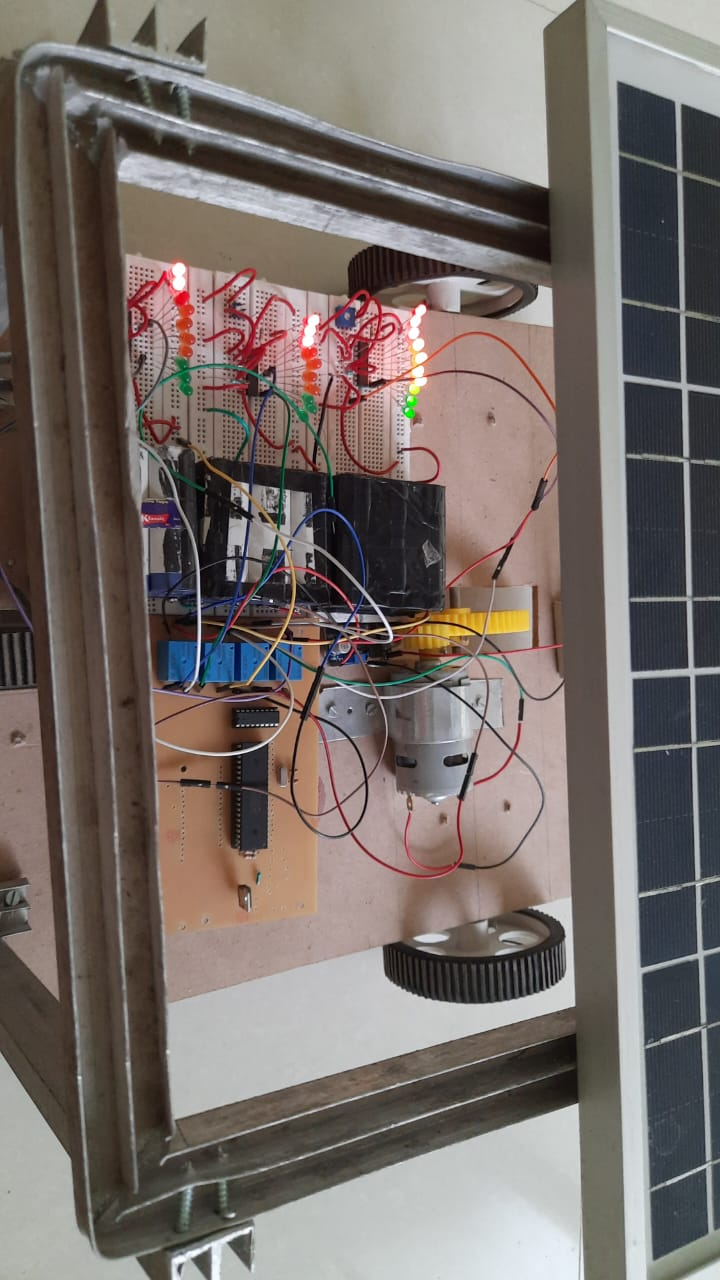
\includegraphics[scale=0.3]{hw4.jpeg}\\
\caption{. Test Stage3}
\end{figure}

Here 3rd battery is discharged and it has started charging.\\

\newpage
\newpage
\thispagestyle{empty}
\vspace*{0.25\textheight}
\begin{center}
\begin{center}
{\bfseries\LARGE <------------------------------------------------------<}\\
{\bfseries\LARGE CHAPTER 5}\\[2cm]


{\scshape\Huge CONCLUSION}\\[0.5cm]
{\scshape\Huge AND}\\[0.5cm]
{\scshape\Huge FUTURE SCOPE}
{\bfseries\LARGE <------------------------------------------------------<}
\end{center}
\end{center}
\newpage

\section{Conclusion and Future Scope}

\subsection{Conclusion}
After completing the project "DESIGN OF SELF CHARGING ELECTRIC VEHICLE USING SOLAR AND WIND POWER" we found that this project can resolve many charging problems of electrical vehicles. 

\subsection{Future Scope}
\begin{itemize}
\item Electric Vehicles are quieter, cleaner and cheaper to operate and maintain, and will last much longer than typical cars.

\item In large scale of equipment would used in Electric Vehicles in future it is useful in various sector like gardening, tourism spot and driving.
\end{itemize}

\newpage
\thispagestyle{empty}
\vspace*{0.25\textheight}
\begin{center}
\begin{center}
{\bfseries\LARGE <------------------------------------------------------<}



{\scshape\Huge REFERENCES}
{\bfseries\LARGE <------------------------------------------------------<}
\end{center}
\end{center}
\newpage
\begin{thebibliography}{REFERENCES}

\bibitem hAerodynamic characterization of a vertical axis wind turbine using a mechatronical experimental setup.Jovencio V. Merin, Caius G. De Guzman, Shawn Michael F./2018
Fabrigar

https://ieeexplore-ieee-org-kkwagh.knimbus.com/document/7547146


\bibitem hHybrid MPPT Solar-Wind Electric Vehicle With Automatic Battery Switching.S. Dupont, IEMN DOAE/2016

https://ieeexplore-ieee-org-kkwagh.knimbus.com/document/8666252


\bibitem kWind Tunnel and Numerical Study of a Small Vertical Axis Wind Turbine.Fadliondi, Haris Isyanto, Budiyanto/2018

https://www.sciencedirect.com/science/article/abs/pii
/S0960148109003048?via


\bibitem kBypass Diodes for Improving Solar Pane Performance.Robert Howell, Ning Qin, Jonathan Edwards, Naveed Durrani/2010

https://www.researchgate.net/publication/330653743

\bibitem lSelf Charging Electric Vehicle.G. H. Chore, K. R. Pandao, R. B. Mode, Y. P. Bagade/2016

\bibitem lDesign And Development of Aerosolar Car.P. A. Bhagat. P. R. Dharme ,P. B. Nikhade, A. L. Wadaskar/2015

\end{thebibliography}

\appendix
\newpage
\thispagestyle{empty}
\vspace*{0.25\textheight}
\begin{center}
\LARGE\textbf{APPENDIX A: Course Detail Sheet}
\addcontentsline{toc}{section}{\numberline{}{APPENDIX A: Course Detail Sheet}}
\end{center}
\newpage
\includepdf[pages=39-41]{ex}
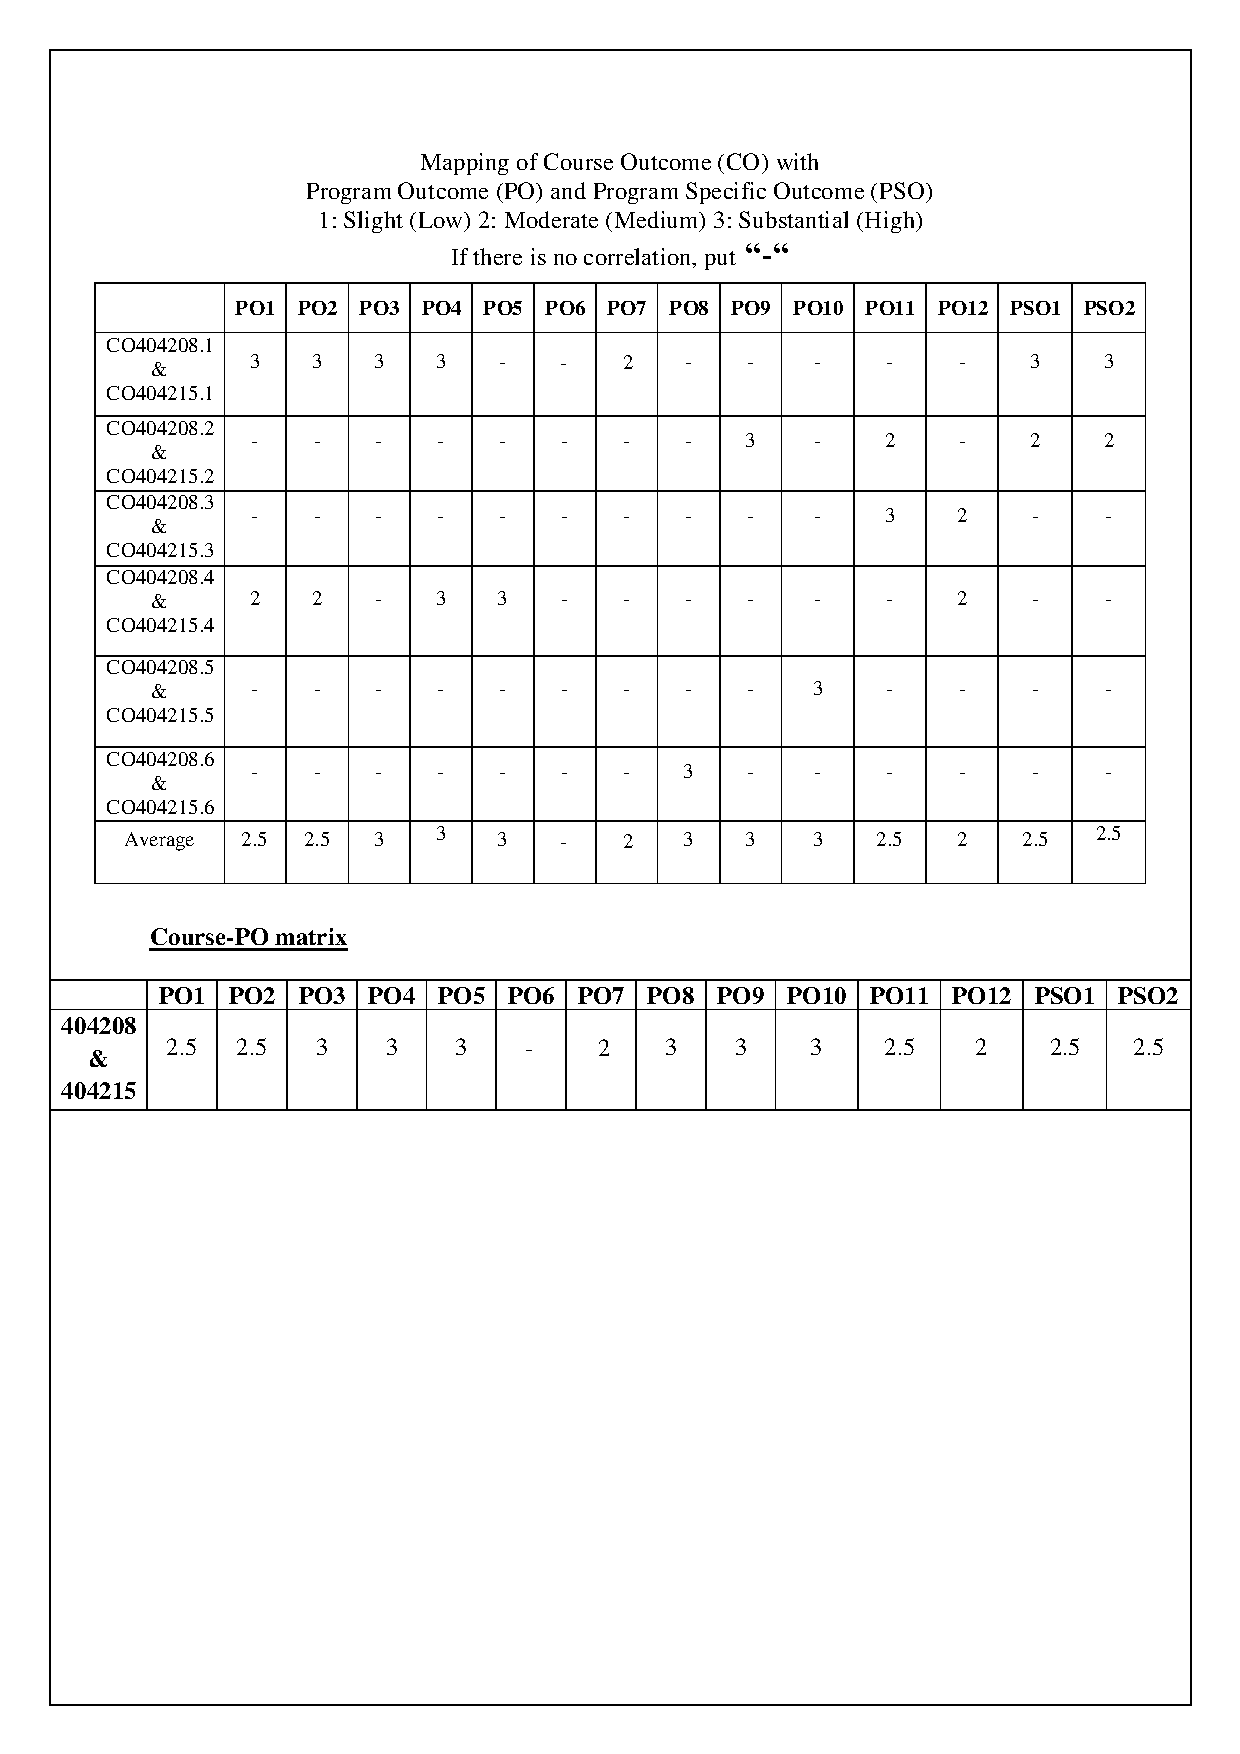
\includepdf[pages={-}]{x}
\newpage

\begin{center}
\LARGE\textbf{APPENDIX B:  Circuit Schematic}
\addcontentsline{toc}{section}{\numberline{}{APPENDIX B:  Circuit Schematic}}
\end{center}

\begin{figure}[!h]
\centering
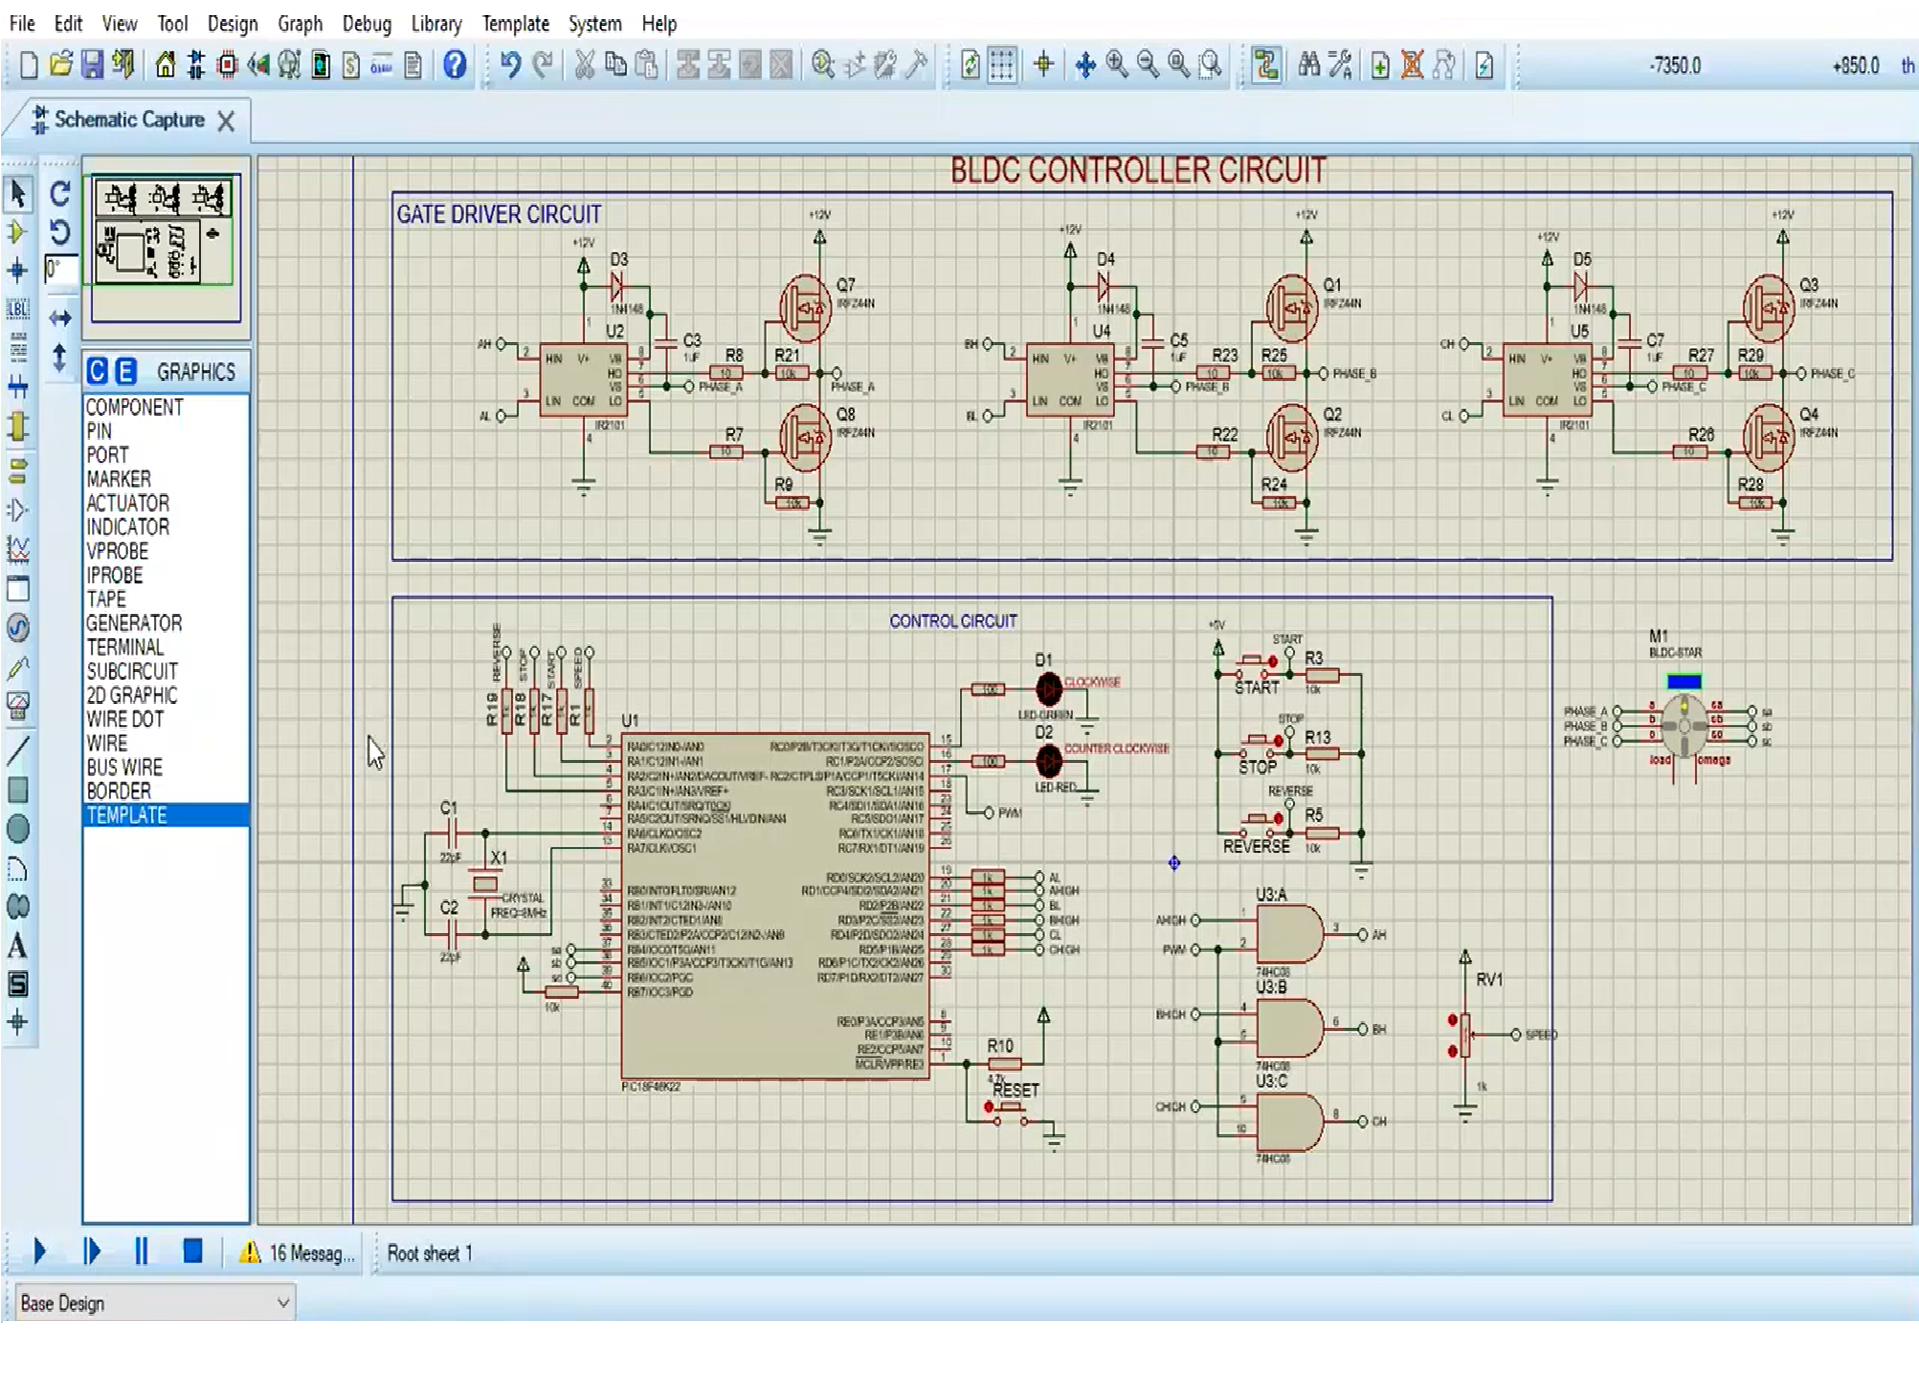
\includegraphics[scale=0.4]{ckt.png}\\
\caption{. BLDC Motor Driver Circuit}
\end{figure}

\begin{figure}[!h]
\centering
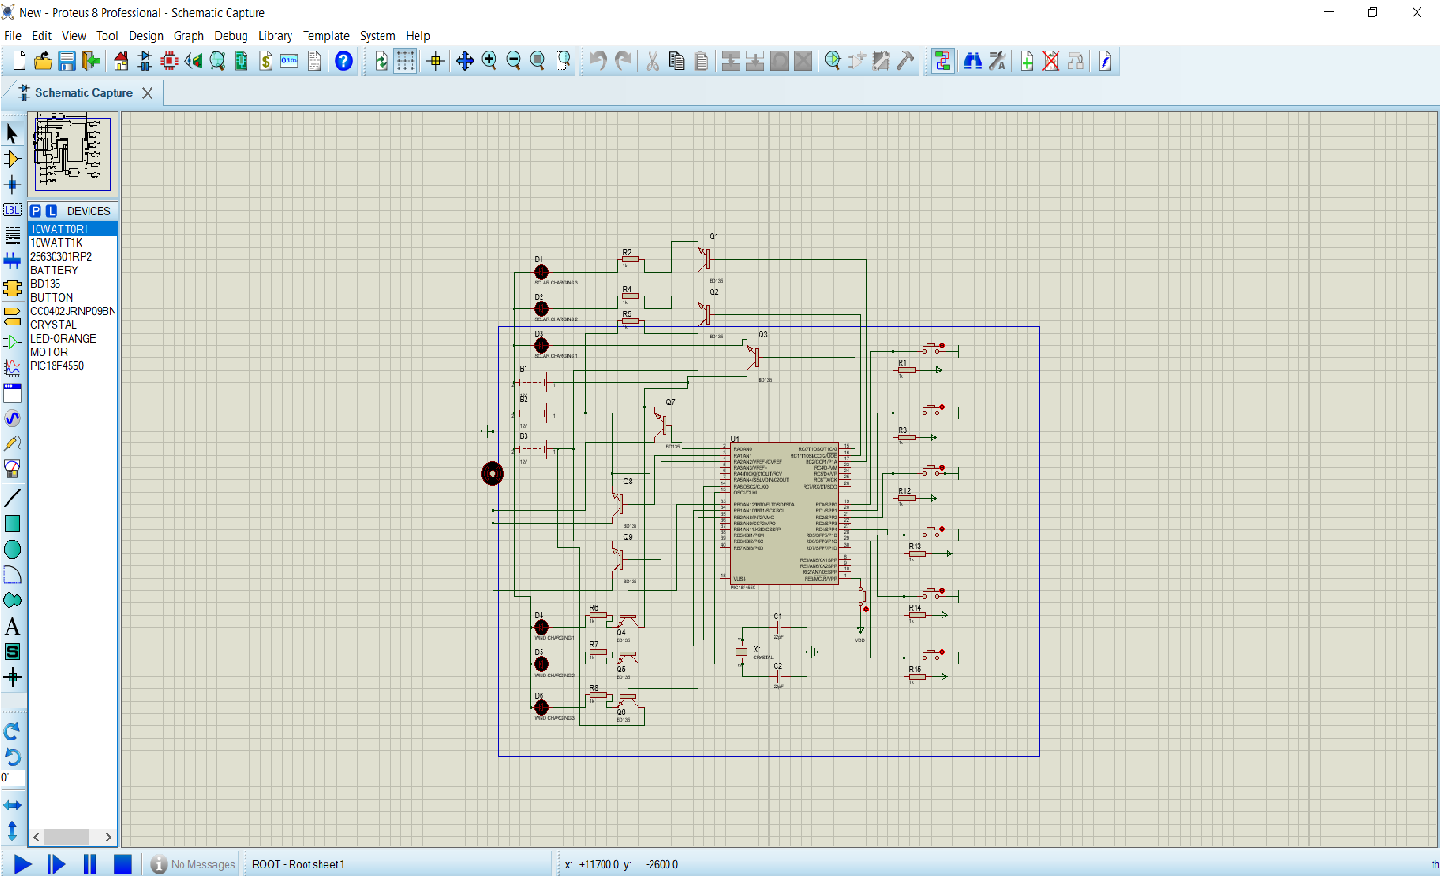
\includegraphics[scale=0.5]{swckt.png}\\
\caption{. Switching Circuit}
\end{figure}

\newpage
\begin{figure}[!h]
\centering
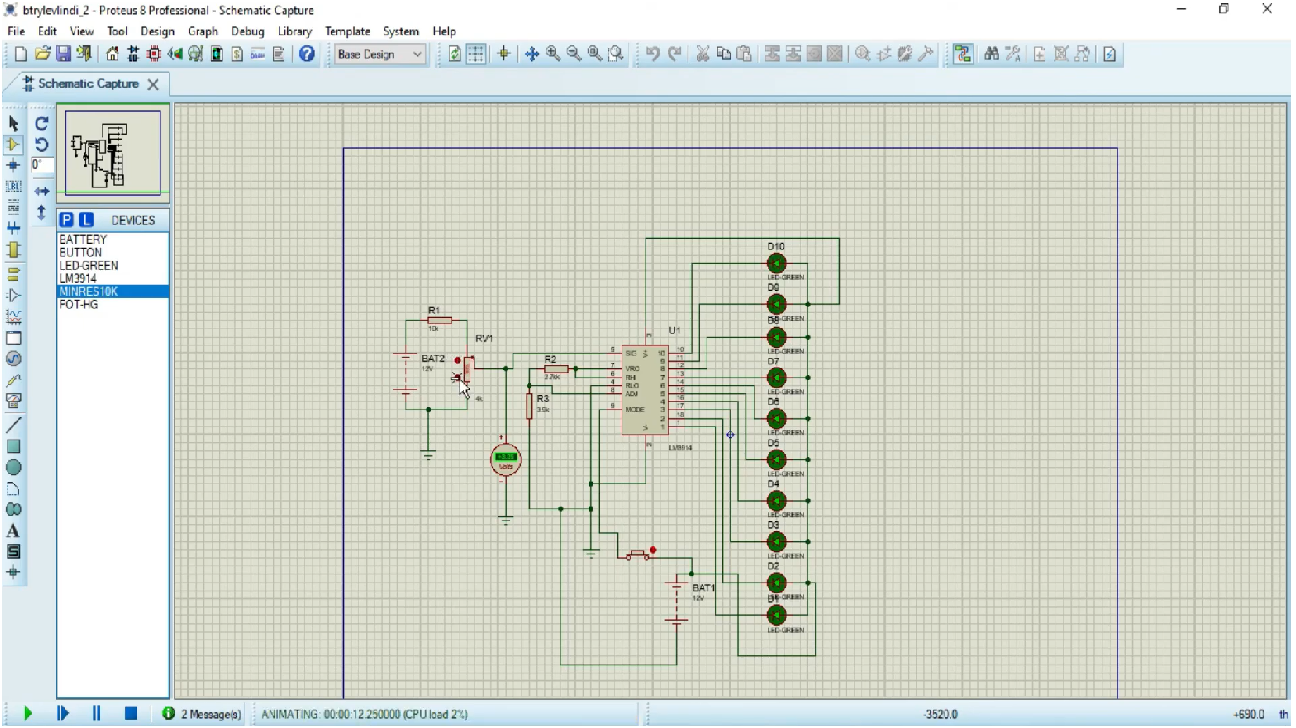
\includegraphics[scale=0.5]{bli.png}\\
\caption{. Battery Level Indicator Circuit}
\end{figure}

\newpage
\begin{center}
\LARGE\textbf{APPENDIX C: Bill of Material}
\addcontentsline{toc}{section}{\numberline{}{APPENDIX C: Bill of Material}}
\end{center}
\begin{table}[!ht]
\centering

\begin{adjustbox}{width=0.7\textwidth}
\begin{tabular}{|c|l|l|p{6cm}|}
\hline
\textbf{Sr No.}
&
\textbf{Components}
&
\textbf{Cost}\\
\hline
1
&
PIC18F4550
&
550/-\\
\hline
2
&
Motors
&
800/-\\
\hline
3
&
Solar Panel
&
1000/-\\
\hline
4
&
Batteries
&
1800/-\\
\hline
5
&
PCB
&
500/-\\
\hline
6
&
IC LM3914
&
200/-\\
\hline
7
&
Opamp
&
50/-\\
\hline
8
&
Others
&
700/-\\
\hline

&
Total
&
5600/-\\
\hline
\end{tabular}
\end{adjustbox}
\caption{Bill of Materials}
\end{table}
\clearpage


\newpage
\thispagestyle{empty}
\vspace*{0.25\textheight}
\begin{center}
\LARGE\textbf{APPENDIX D: Certificate of Paper Presentation/Project Competition}
\addcontentsline{toc}{section}{\numberline{}{APPENDIX D: Certificate of Paper Presentation/Project Competition}}
\end{center}
\newpage

\includepdf[pages={-}]{hr}
\newpage

\includepdf[pages={-}]{sm}
\newpage

\includepdf[pages={-}]{st}

\newpage
\begin{center}
\LARGE\textbf{APPENDIX E: Report for Plagiarism Check}
\addcontentsline{toc}{section}{\numberline{}{APPENDIX E: Report for Plagiarism Check}}\\[1cm]
\end{center}
\thispagestyle{empty}
\begin{center}
\textbf{\LARGE\scshape\underline{Plagiarism Certificate}}\\[2cm]
\addcontentsline{toc}{subsection}{\numberline{}{Plagiarism Certificate}}
\end{center}
\large This is to certify that the project work titled \textbf{“DESIGN OF SELF CHARGING ELECTRIC VEHICLE USING SOLAR AND WIND POWER"}, is a part of project work carried out by \textbf{“Hrugved Manbhekar, Shreyash Modak and Saurav Tayade”}
under the guidance of\textbf{ Prof R.R.Khinde} at K. K. Wagh Institute of
Engineering Education and Research, Nashik, in the partial fulfillment of the requirements
for Bachelor’s degree in Electronics and Telecommunication Engineering.\\
\large To the best of our knowledge, the work included in this report is an original work
carried out by us independently. The percentage of plagiarism is 6 percent. The results of the
project work in part or whole have not been submitted to any other Institute/University for
the award of any degree.

\vspace{4cm}
\begin{flushright}
Hrugved Manbhekar\\
Shreyash Modak\\
Saurav Tayade\\

B.E. Electronics\\
\end{flushright}

\newpage
\begin{figure}[!h]
\centering
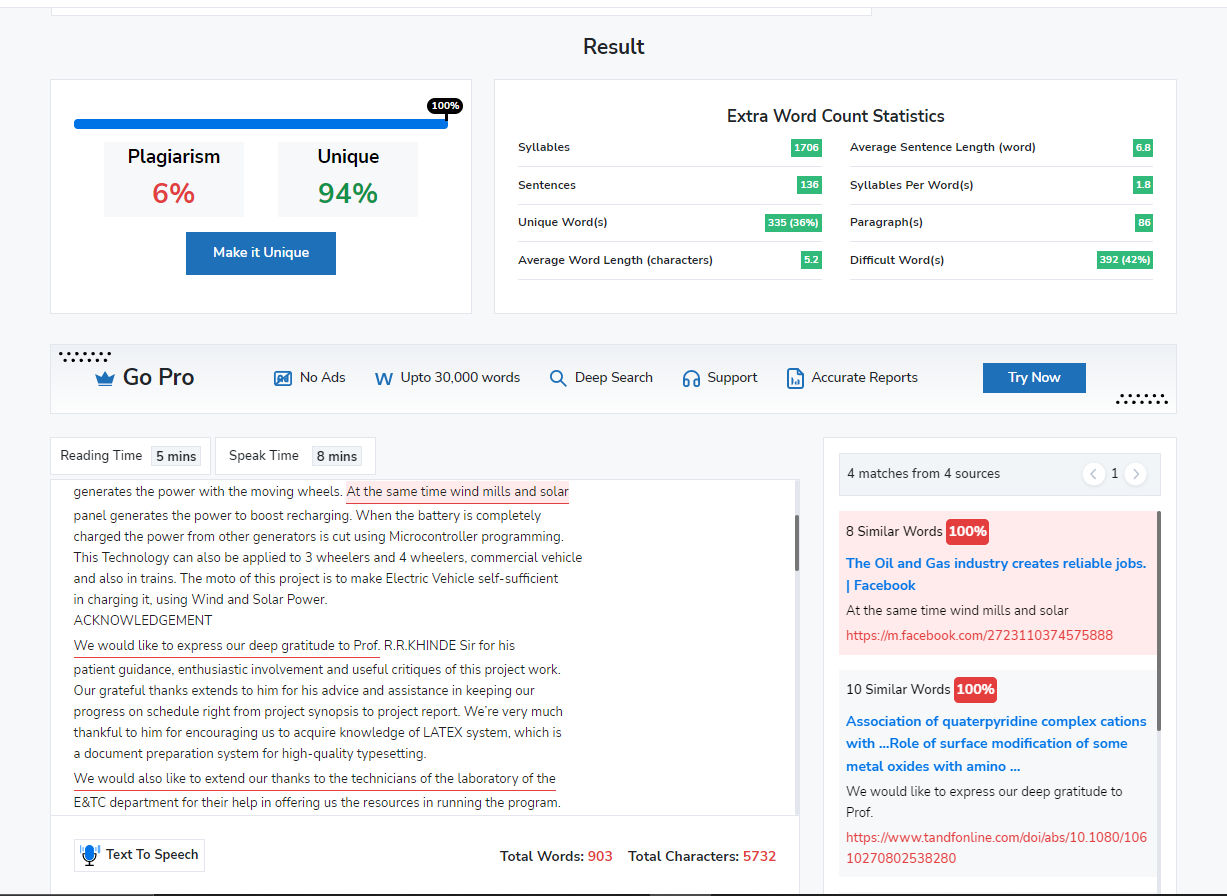
\includegraphics[scale=0.5]{pl.png}\\
\caption{. Plagiarism Result}
\end{figure}


\newpage
\thispagestyle{empty}
\vspace*{0.25\textheight}
\begin{center}
\LARGE\textbf{APPENDIX F:  Data Sheets}
\addcontentsline{toc}{section}{\numberline{}{APPENDIX F:  Data Sheets}}
\end{center}

\newpage
 PIC18F4550 Datasheet
\begin{figure}[!h]
\centering
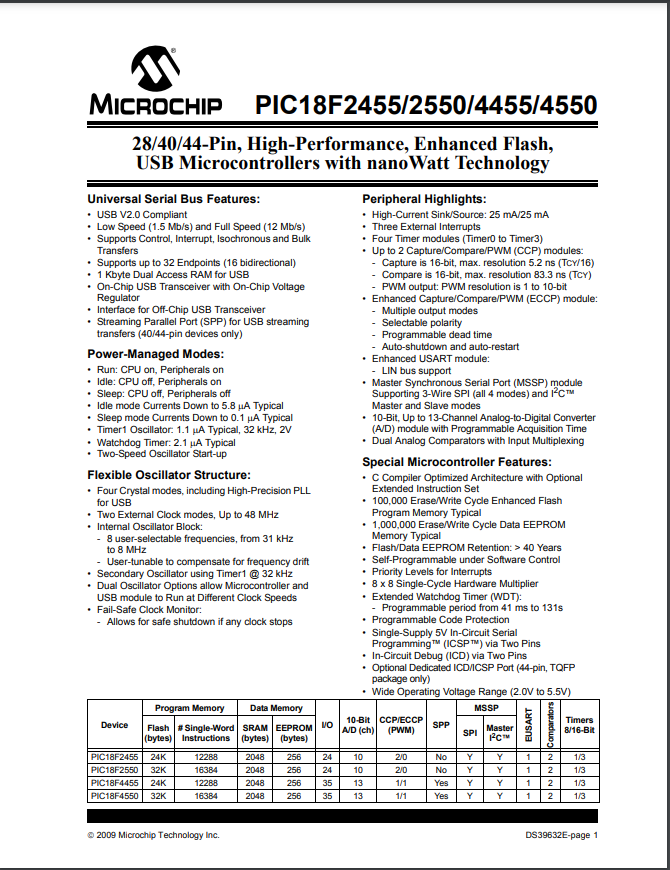
\includegraphics[scale=1.2]{pic18datasheet.png}\\
\end{figure}

\newpage
 Solar PV  Module Datasheet
\begin{figure}[!h]
\centering
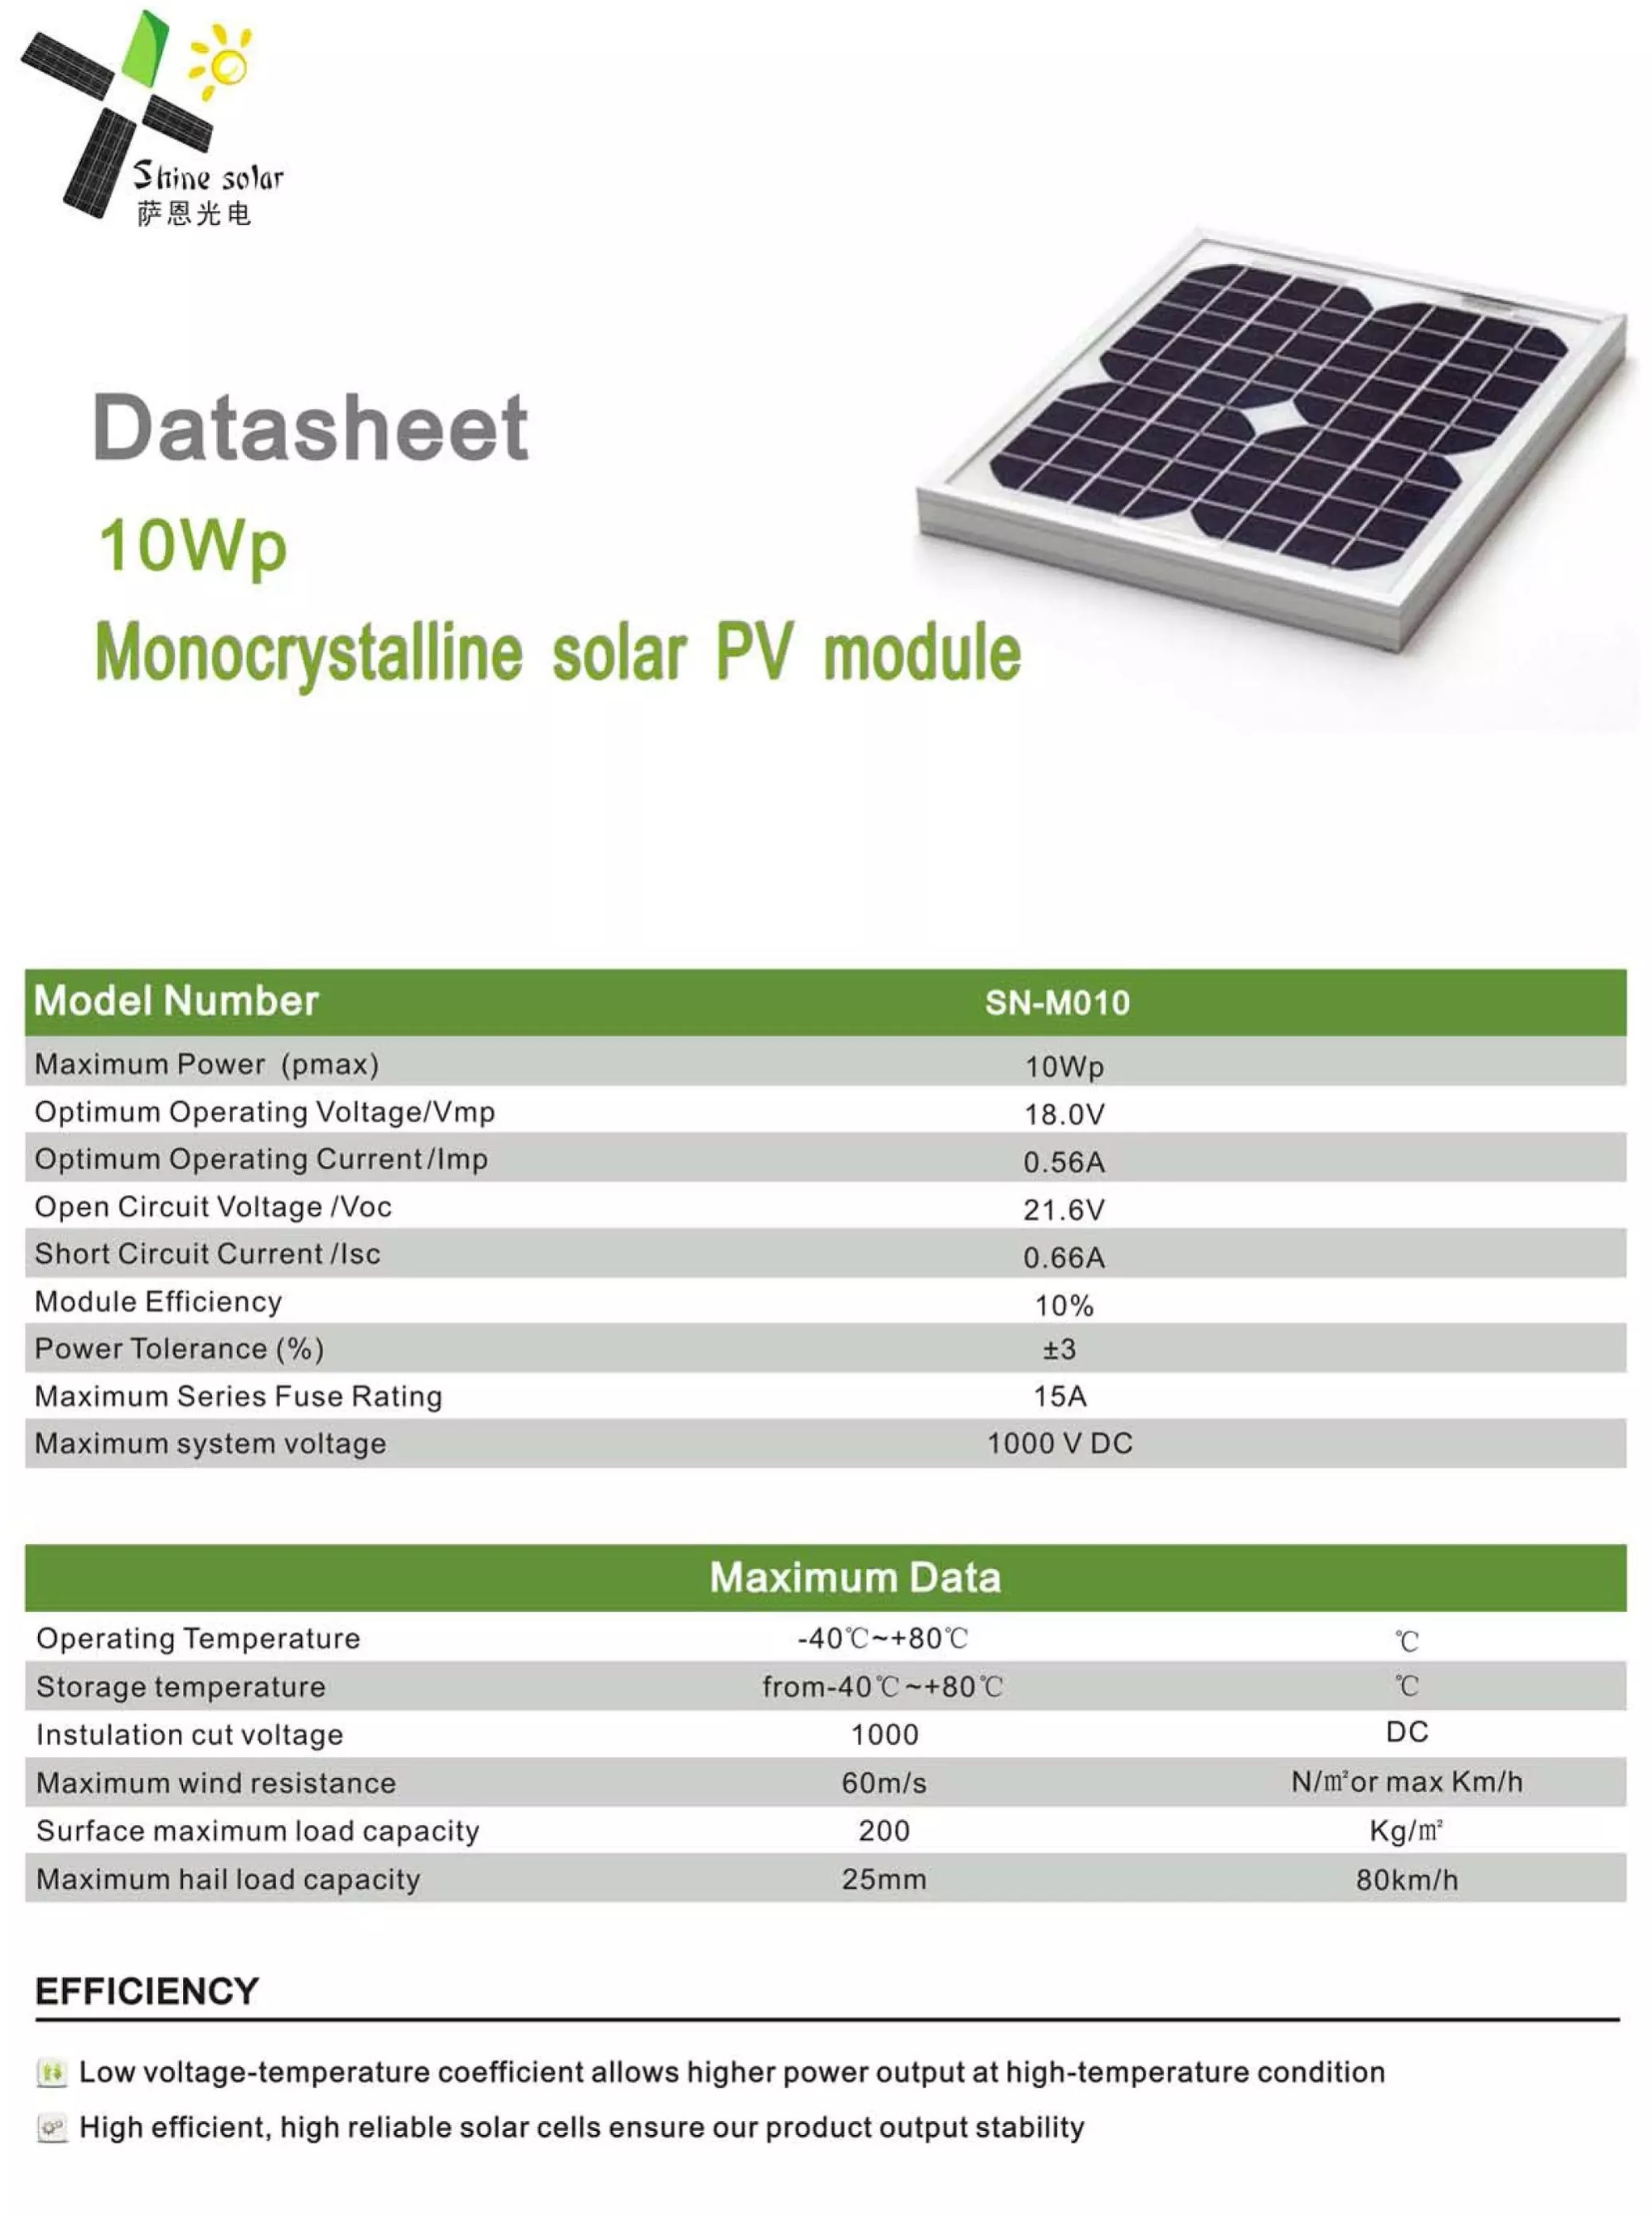
\includegraphics[scale=0.4]{PV.jpg}\\
\end{figure}


\newpage
DC Motor Datasheet
\begin{figure}[!h]
\centering
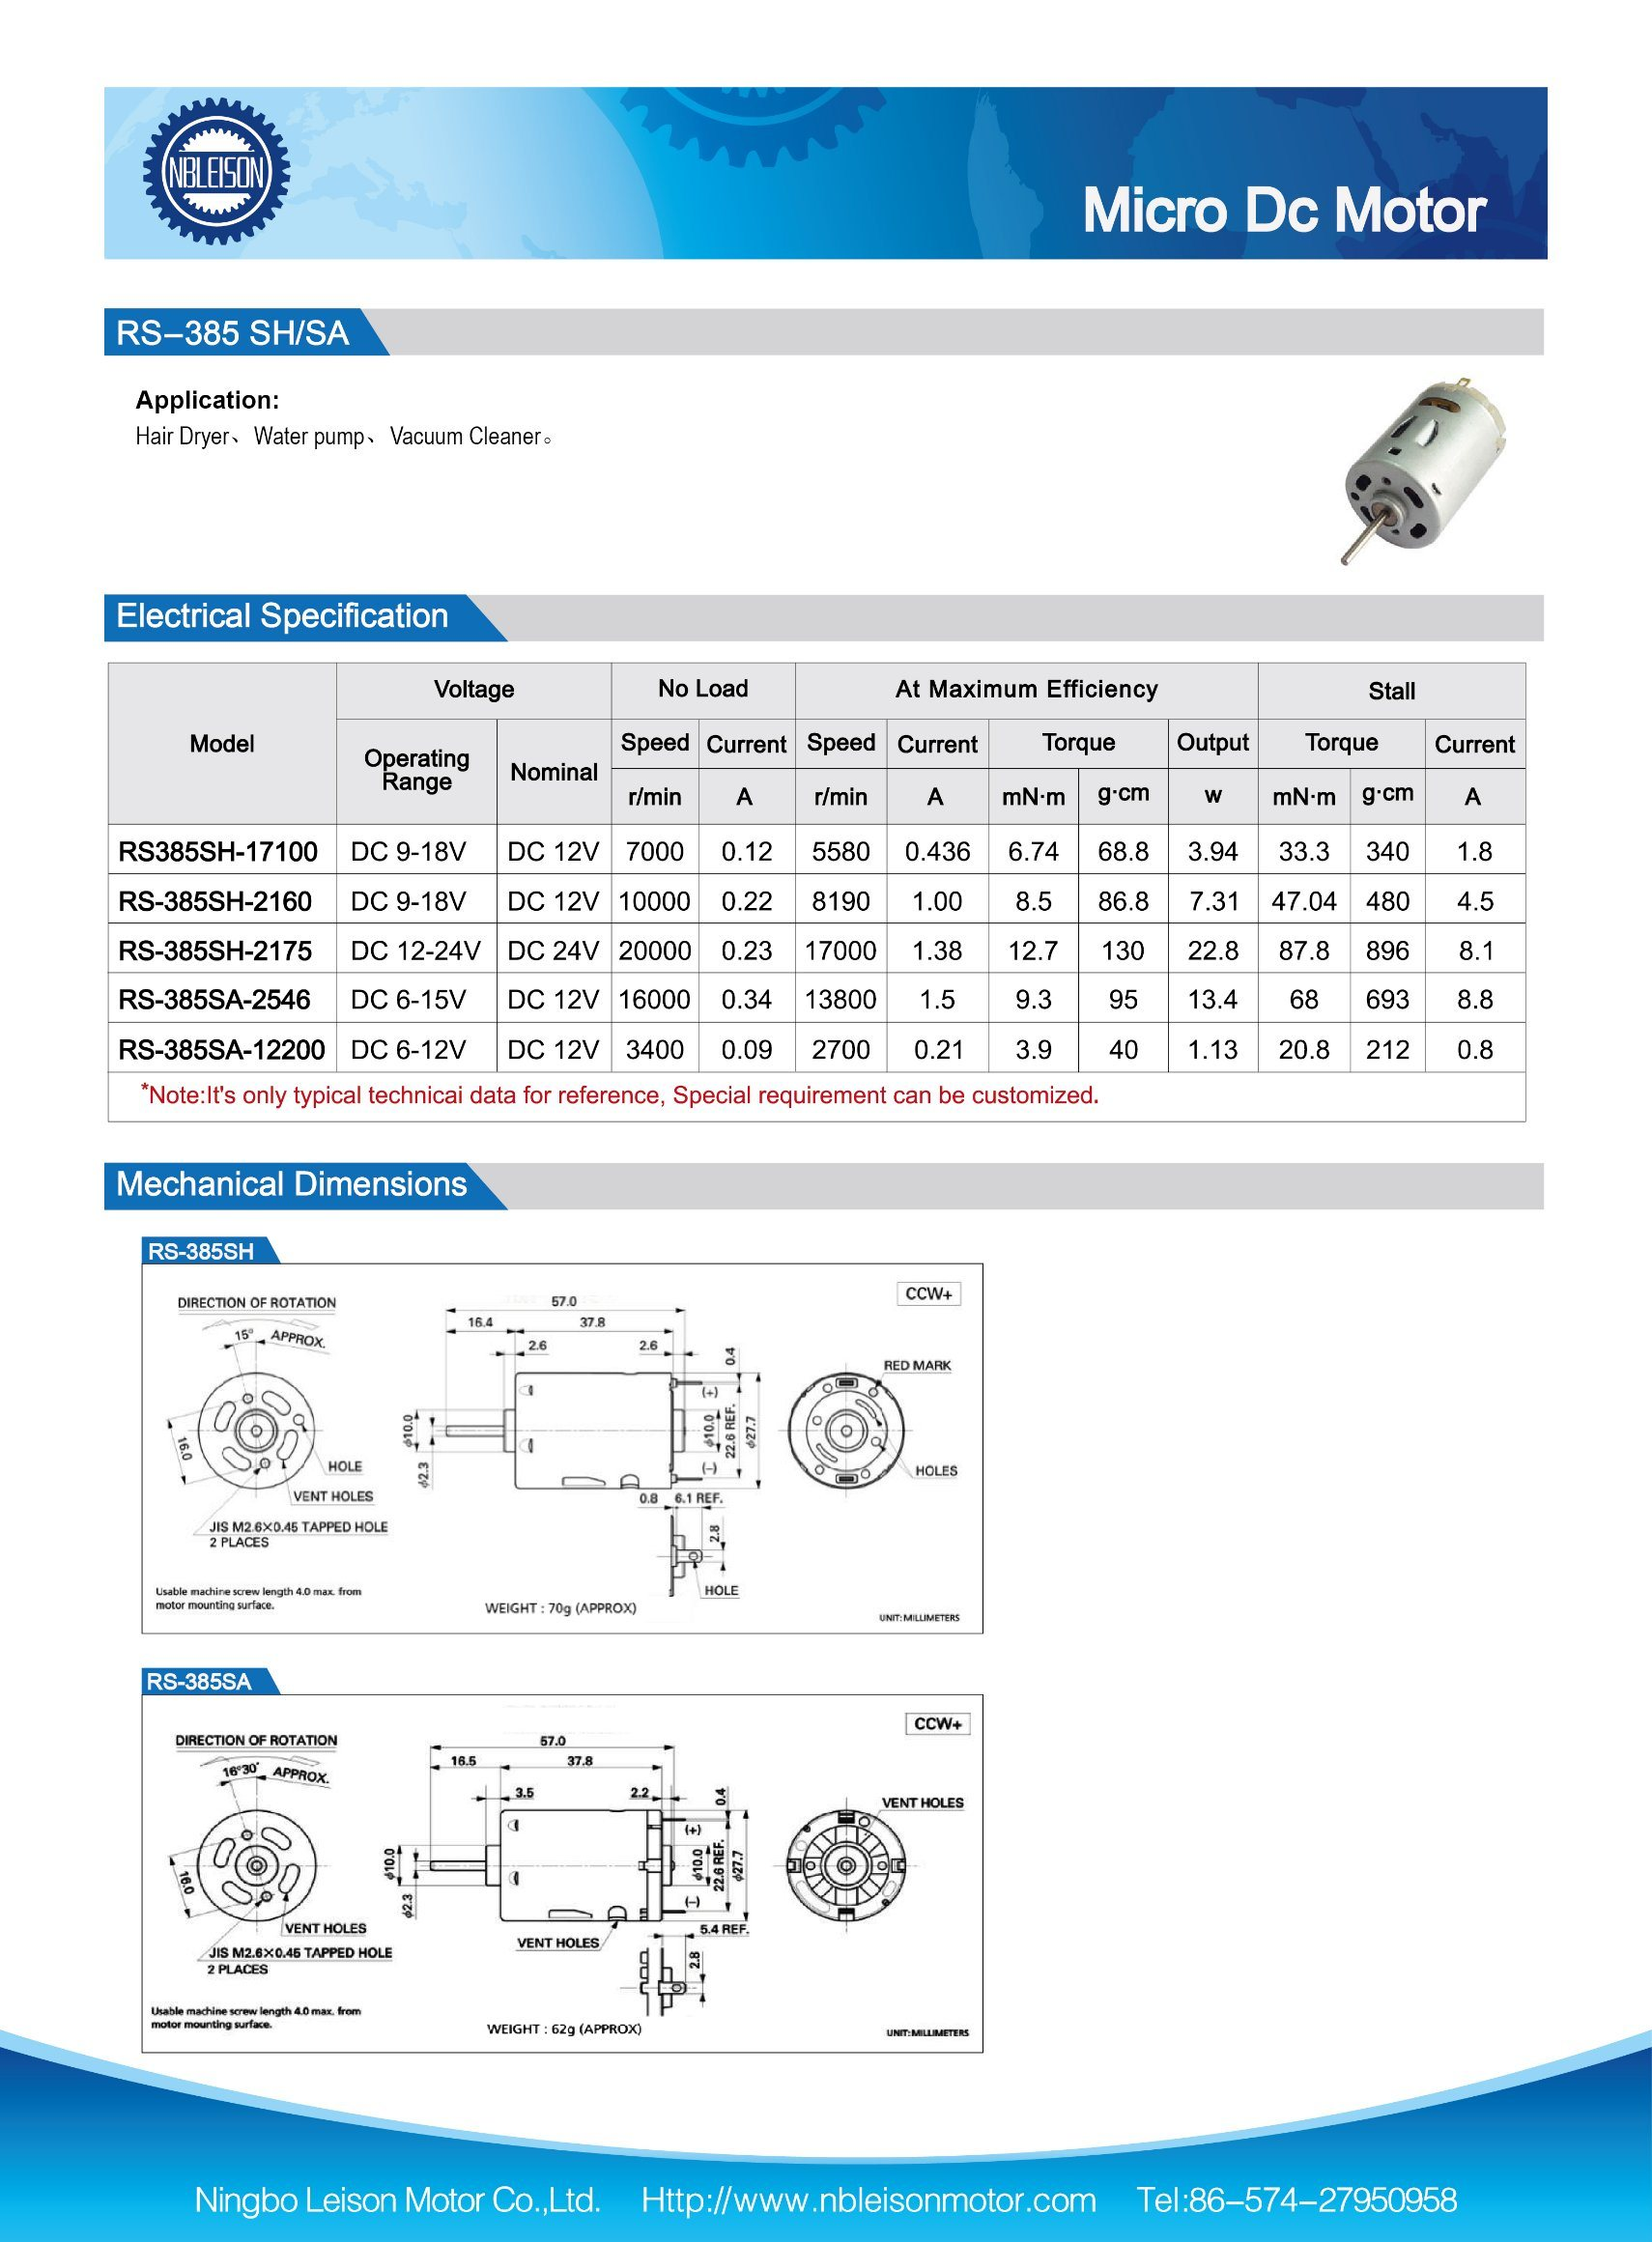
\includegraphics[scale=0.28]{dcm.jpg}\\
\end{figure}


\newpage
\thispagestyle{empty}
\vspace*{0.25\textheight}
\begin{center}
\LARGE\textbf{APPENDIX G:  Rubrics for Project Phase-I and Phase-II}
\addcontentsline{toc}{section}{\numberline{}{APPENDIX G:  Rubrics for Project Phase-I and Phase-II}}
\end{center}

\newpage
\includepdf[pages=59-63]{ex}


\enddocument